\documentclass[10pt,xcolor={dvipsnames}]{beamer}
\usetheme[
%%% option passed to the outer theme
%    progressstyle=fixedCircCnt,   % fixedCircCnt, movingCircCnt (moving is deault)
  ]{Feather}
  
% If you want to change the colors of the various elements in the theme, edit and uncomment the following lines

% Change the bar colors:
\setbeamercolor{Feather}{fg=NavyBlue!20,bg=NavyBlue}

% Change the color of the structural elements:
\setbeamercolor{structure}{fg=NavyBlue}

% Change the frame title text color:
\setbeamercolor{frametitle}{fg=black!5}

% Change the normal text colors:
\setbeamercolor{normal text}{fg=black!75,bg=gray!5}

%% Change the block title colors
\setbeamercolor{block title}{use=Feather,bg=Feather.fg, fg=black!90} 


% Change the logo in the upper right circle:
%\renewcommand{\logofile}{example-grid-100x100pt} 
%% This is an image that comes with the LaTeX installation
% Adjust scale of the logo w.r.t. the circle; default is 0.875
% \renewcommand{\logoscale}{0.55}

% Change the background image on the title and final page.
% It stretches to fill the entire frame!
% \renewcommand{\backgroundfile}{example-grid-100x100pt}

%-------------------------------------------------------
% INCLUDE PACKAGES
%-------------------------------------------------------

\usepackage[utf8]{inputenc}
\usepackage[english]{babel}
\usepackage[T1]{fontenc}
\usepackage{amsfonts}
% \usepackage{helvet}

%% Load different font packages to use different fonts
%% e.g. using Linux Libertine, Linux Biolinum and Inconsolata
 %\usepackage{libertine}
% \usepackage{zi4}

%% e.g. using Carlito and Caladea
%\usepackage{carlito}
%\usepackage{caladea}
\usepackage{amssymb, amsmath, amsthm}
\usepackage{zi4}
\graphicspath{ {figures/}{figures/eps/}{figures/pdf/} }% specify the path where figures are located
\usepackage{amsmath}
\usepackage{amscd,latexsym,amsfonts,amstext,amsbsy}
\usepackage[mathscr]{euscript} %for european script
\usepackage{colortbl}
\usepackage{graphics}
\usepackage{graphicx}
\usepackage{epstopdf}
\usepackage{amssymb}
\usepackage{amsmath}
\usepackage{cite}
\usepackage{color,soul}
\usepackage{array}
\usepackage{xcolor}
\newcolumntype{C}[1]{>{\centering\let\newline\\\arraybackslash\hspace{0pt}}m{#1}}
\usepackage[config, labelfont={bf}]{caption,subfig}
\usepackage{float}
\usepackage{caption}
\usepackage{comment}
\newcolumntype{K}[1]{>{\centering\arraybackslash}p{#1}}



%% e.g. using Venturis ADF Serif and Sans
% \usepackage{venturis}

%-------------------------------------------------------
% DEFFINING AND REDEFINING COMMANDS
%-------------------------------------------------------

% colored hyperlinks
\newcommand{\chref}[2]{
  \href{#1}{{\usebeamercolor[bg]{Feather}#2}}
}






\newenvironment<>{varblock}[2][\textwidth]{%
  \setlength{\textwidth}{#1}
  \begin{actionenv}#3%
    \def\insertblocktitle{#2}%
    \par%
    \usebeamertemplate{block begin}}
  {\par%
    \usebeamertemplate{block end}%
  \end{actionenv}}


  
  
  
\begin{document}
\newcommand{\cfbox}[2]{%
    \colorlet{currentcolor}{.}%
    {\color{#1}%
    \fbox{\color{currentcolor}#2}}%
}




\title[] % [] is optional - is placed on the bottom of the sidebar on every slide
{ % is placed on the title page
      {\textbf{Modeling the Heroin Epidemic: \\A Preliminary Report}}
}

\subtitle[SIAM Annual Meeting 2018]
{
      
}

\author[T. Phillips]
{    \large{Presented by: Tricia Phillips, University of Tennessee, Knoxville} \\ 
\vspace{0.5cm}
Collaborators: Dr. Suzanne Lenhart and \\ Dr. Christopher Strickland 
      %{\ttfamily lilqna.v@gmail.com}\\[1em]
      %with v1.1 modifications by LianTze Lim (Overleaf)
}


%\institute{Dissertation Defense}
%{%
   %   Faculty of Mathematics, Informatics and Information Technologies\\
     % Plovdiv University ``Paisii Hilendarski''
%}

%\date{\today}
\date{July 10, 2018}


%\title[Optimal Control of Vacc for \textit{C. diff}]{Optimal Control of Vaccination Rate in an Epidemiological Model of \textit{Clostridium difficile} Transmission} 
%\author[Stephenson]{Brittany Stephenson \\
 %Cristina Lanzas\\
%Suzanne Lenhart\\
%Judy Day}
%\institute[UTK]{ University of Tennessee, Knoxville\\ }
%\date{\today}
  
 



{\1% % this is the name of the PDF file for the background
\begin{frame}[plain,noframenumbering] % the plain option removes the header from the title page, noframenumbering removes the numbering of this frame only
  \titlepage % call the title page information from above
\end{frame}}
  
  
\begin{frame}{Content}{}
\frametitle{Overview}
\tableofcontents
\end{frame}
  
  
\section{Motivation for Heroin Model}



\begin{frame}
\frametitle{Motivation}
{\color{beamer@headercolor}  \textbf{Opioids}} 

\begin{itemize}

\item<1> The misuse of opioids, a drug class including prescription pain relievers and heroin, is rampant in today's society.
\item<1> Number of opioid prescriptions that pharmacies distributed tripled from 1991 to 2011. 
\item<1> Dramatic increase in accessibility to heroin and the lower cost of the drug has influenced prescription opioid users to turn to heroin.
\item<1> Estimated 80\% of heroin users at the national level used prescription opioids previously. 
\item<1> The opioid crisis was declared a public health emergency in October 2017 by the United States Department of Health and Human Sciences.
\end{itemize}


\end{frame}





\begin{frame}
\frametitle{Motivation}


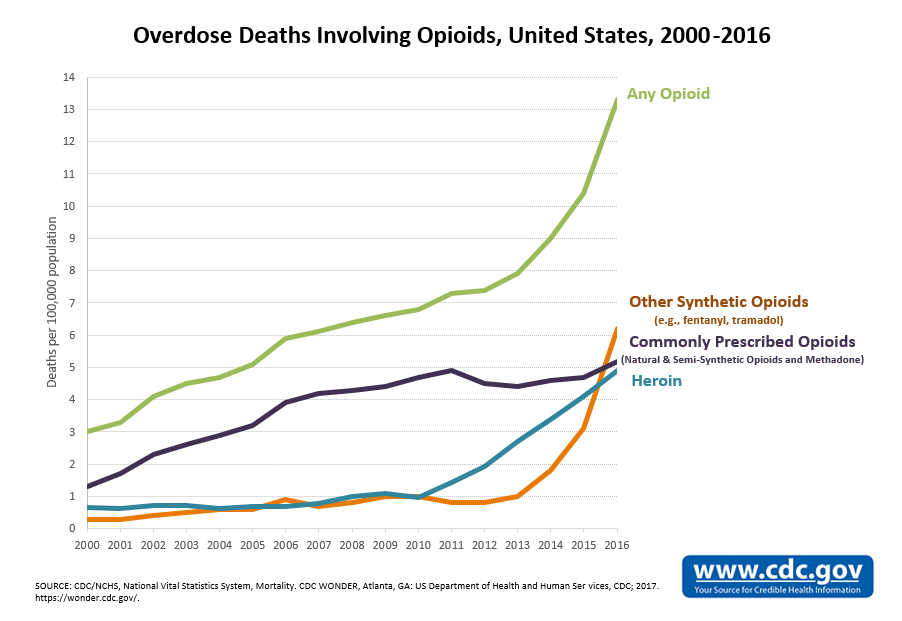
\includegraphics[height=6cm, width=11cm]{opioid_overdoses.png}


\begin{center}
\textbf{Source:} Centers for Disease Control and Prevention 
\end{center}
\end{frame} 






\begin{frame}
\frametitle{Motivation}
\vspace{-1cm}
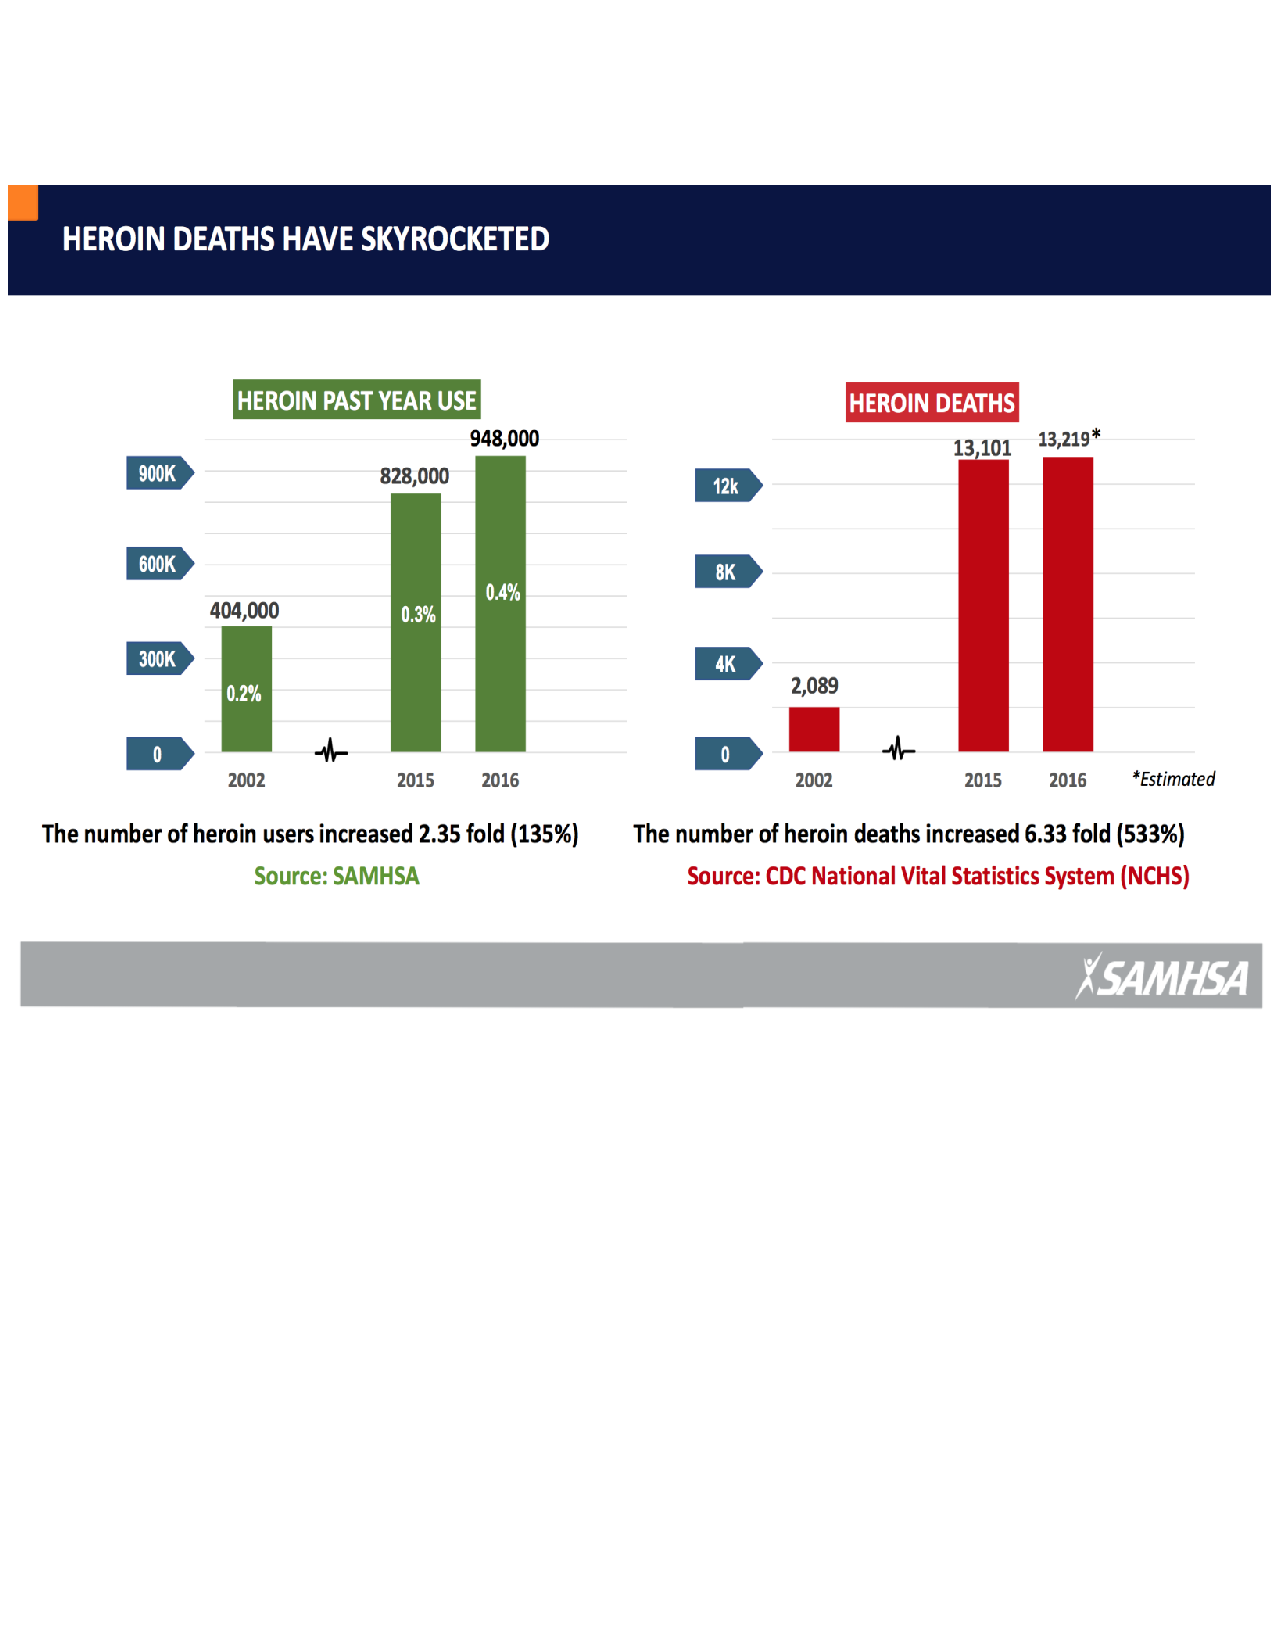
\includegraphics[height=12cm, width=11cm]{heroin_deaths.pdf}
 \vspace{-5cm}

\begin{center}
\textbf{Source:}  2016 National Survey on Drug Use and Health Report from SAMSHA.gov
\end{center}
\end{frame} 


\section{Heroin Model Formulation}  
  
 \begin{frame}
\frametitle{Model Formulation}
\begin{itemize}
\item {\color{beamer@headercolor}  \textbf{Goals}}: 
\vspace{0.3cm}
\begin{enumerate}[-]
\item Investigate the dynamics behind the opioid  (non-heroin) and heroin epidemic and identify important conditions relating to the reduction of opioid and heroin addicted individuals. 
\vspace{.2cm}
\item Develop a system of ODEs model consisting of classes of individuals taking prescription opioids, addicted to opioids, using heroin and recovering from opioid addiction, including heroin, and analyze it. 
\vspace{.2cm}
\item Investigate management strategies for how to best treat pain with prescriptions while reducing opioid addiction and heroin use. 
\end{enumerate}
\end{itemize}

\end{frame}
  
  
  
  
  
   \begin{frame}
\frametitle{Model Formulation}

\begin{itemize}
\item[-]<1> Based on work by Battista, Pearcy, Strickland (preprint 2018). 
\item[-]<1> Formulated a five class compartmental population model (classes are fractions of the entire population). 

\item[-]<1> {\color{beamer@headercolor} Population Classes} 
\begin{itemize}
\item[-]<1> Susceptibles ($S$): not taking prescription opioids, nor using heroin. \\
\item[-]<1> Prescription opioid users ($P$): opioid-prescribed individuals not considered addicted. 
\item[-]<1>  Opioid addicts ($A$): addicted to opioids. 
\item[-]<1> Heroin users ($H$): addicted to heroin. 
\item[-]<1> Individuals in treatment/rehabilitation ($R$): undergoing treatment for their addiction to opioids or heroin. 

\end{itemize}
\end{itemize}

\end{frame}




\begin{frame}
\frametitle{}
\vspace{-.52cm}
\hspace*{-1.08cm} 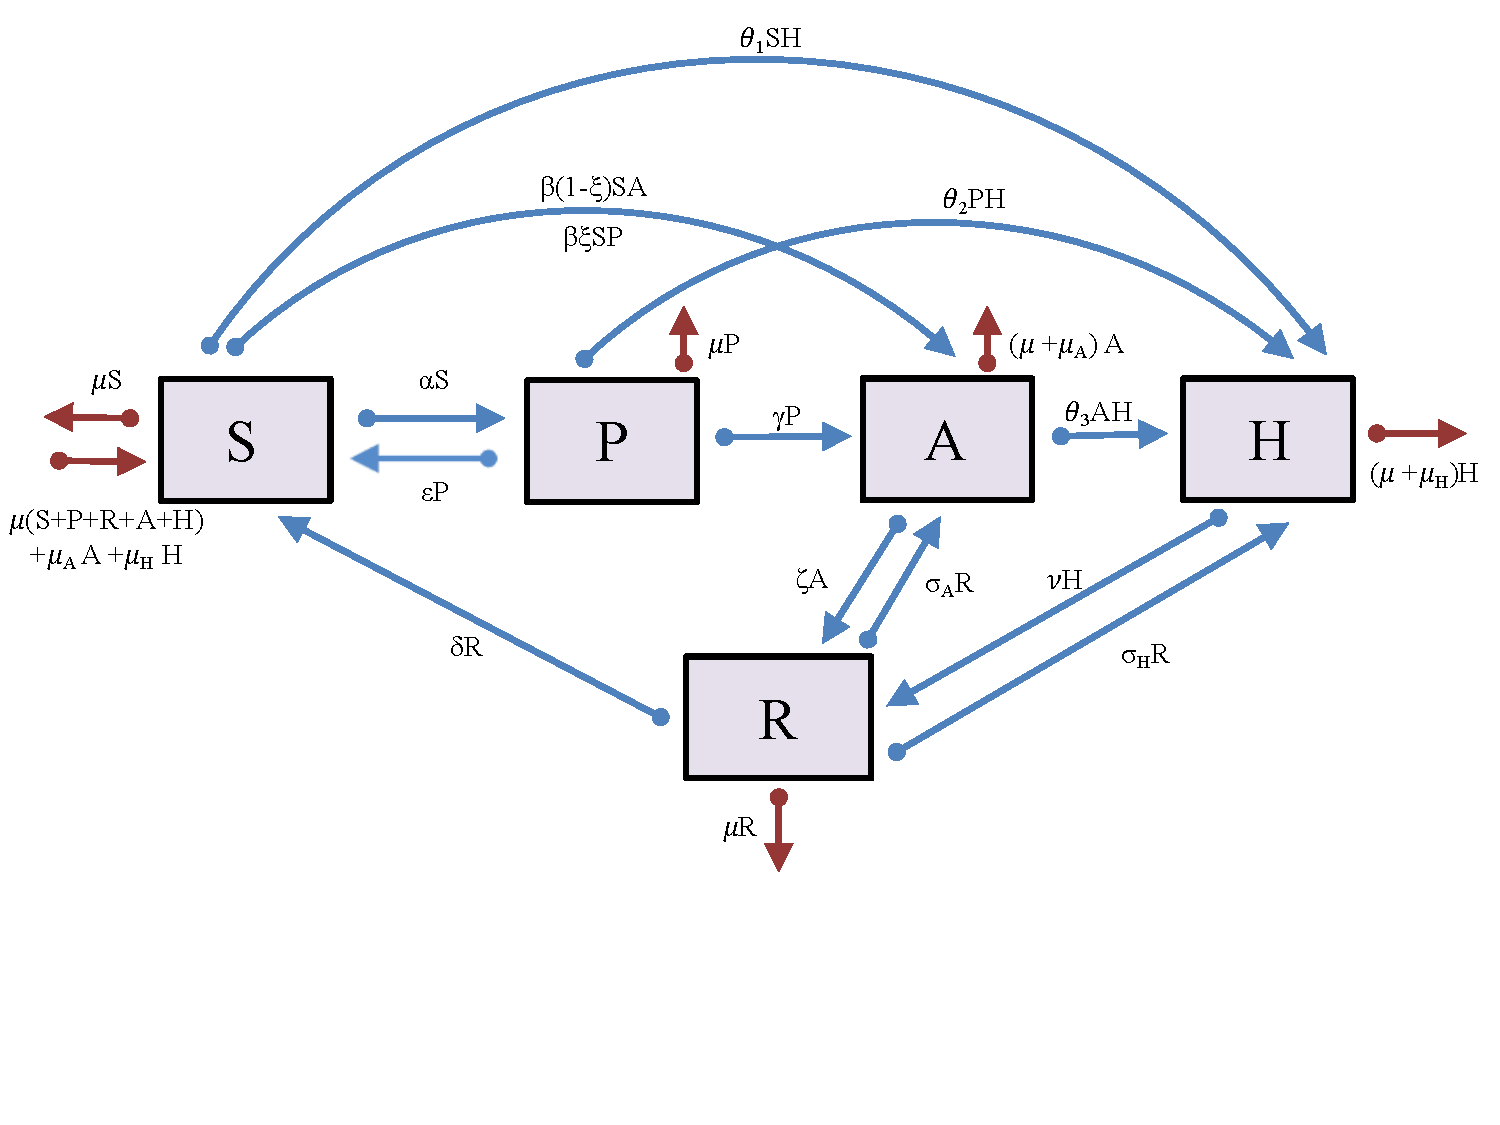
\includegraphics[height=7.5cm, width=12.8cm]{heroin_schematic.pdf} \hspace*{4.5cm}
\begin{center}
$\alpha S$: prescription rate 
\end{center}
\end{frame}


\begin{frame}
\frametitle{}
\vspace{-.28cm}
\hspace*{-1.08cm} 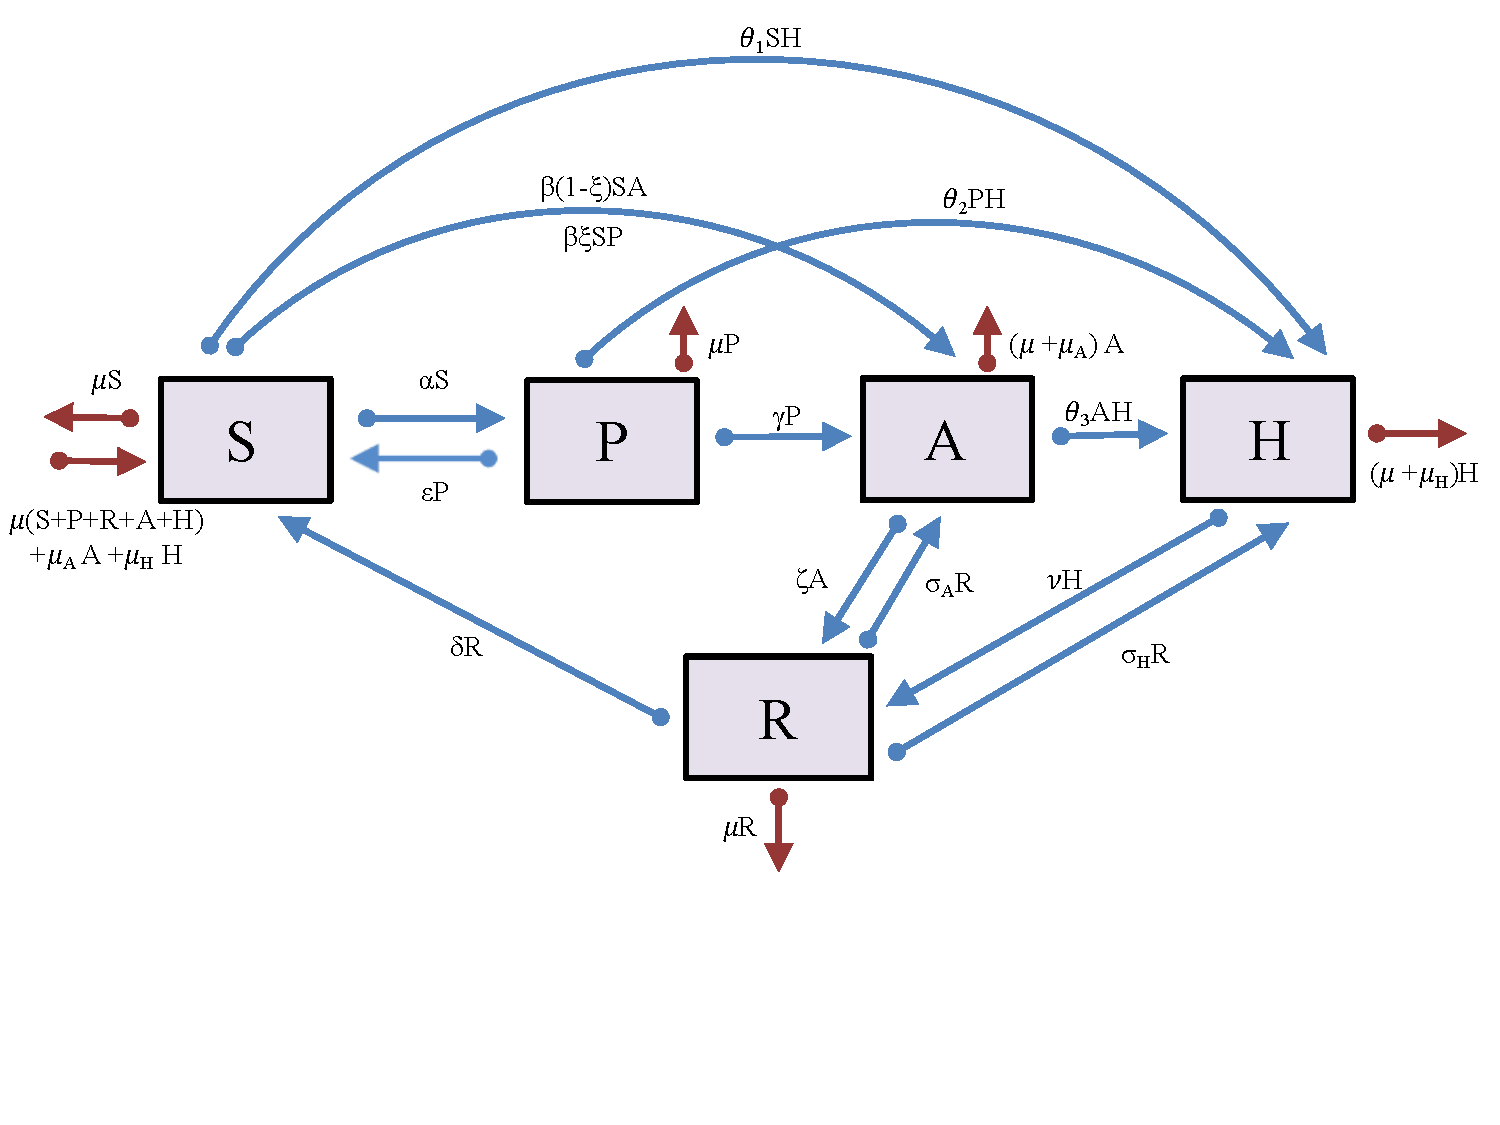
\includegraphics[height=7.5cm, width=12.8cm]{heroin_schematic.pdf} \hspace*{4.5cm}
\begin{center}
$\beta(1-\xi)SA$: opioid addiction rate by black market drugs/interaction with other addicts 
\end{center}
\end{frame}




\begin{frame}
\frametitle{}
\vspace{-.52cm}
\hspace*{-1.08cm} 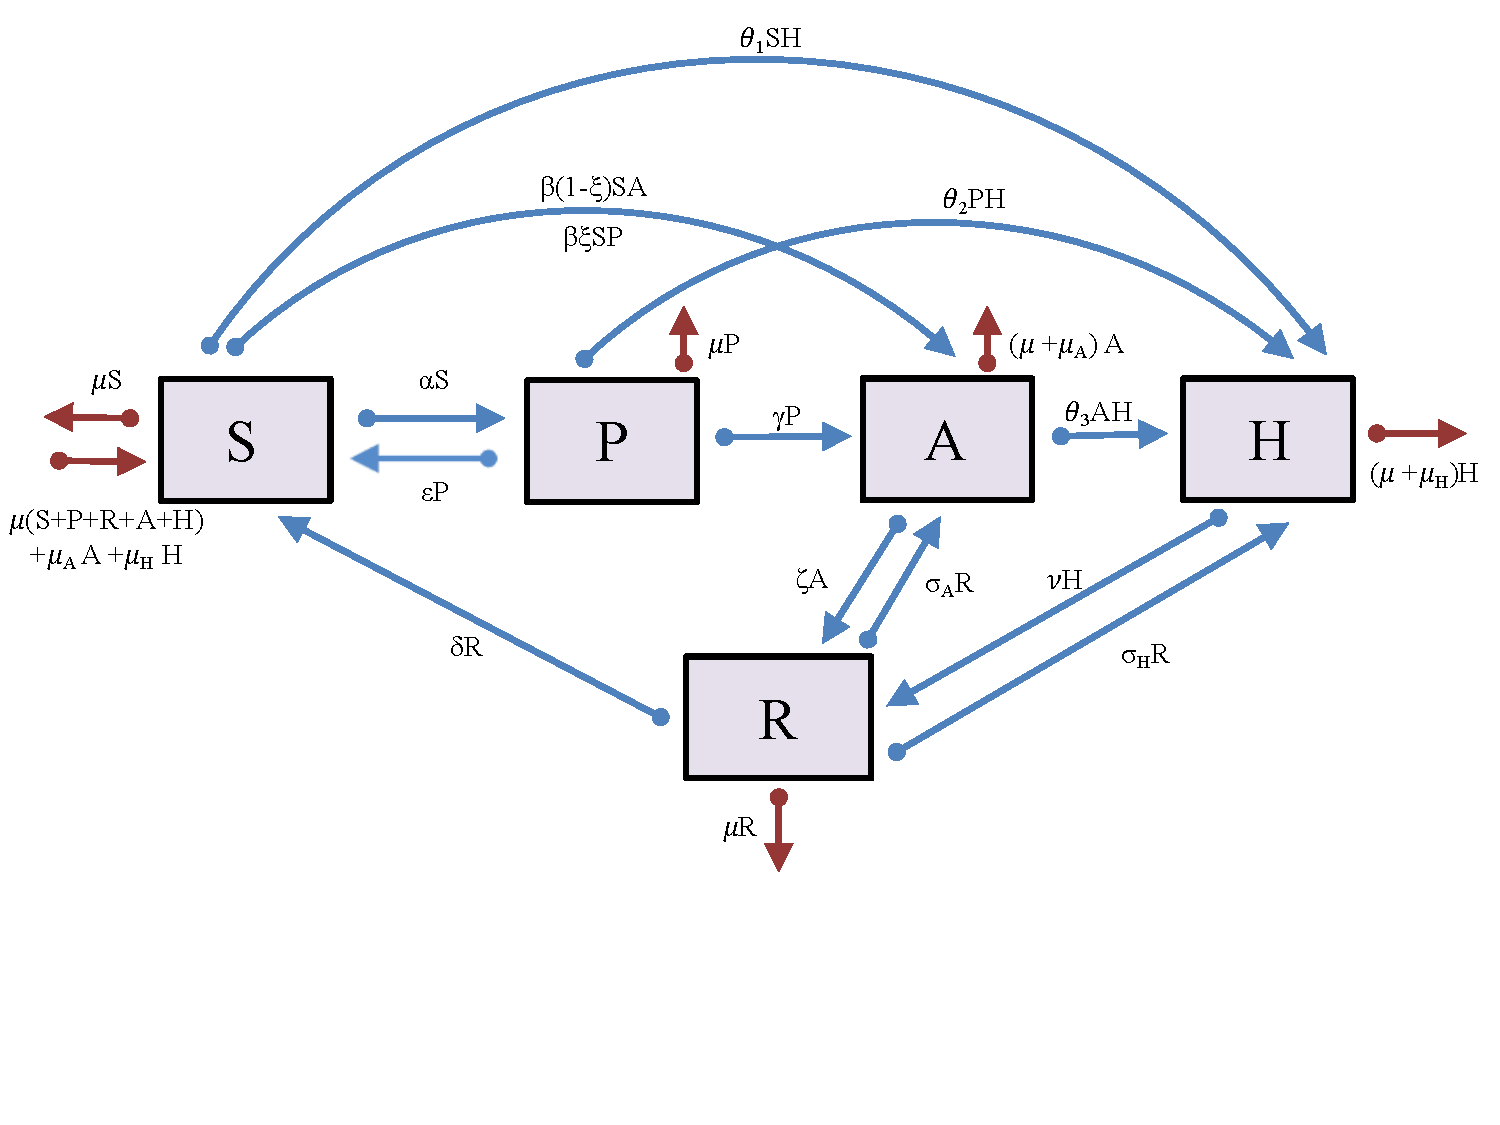
\includegraphics[height=7.5cm, width=12.8cm]{heroin_schematic.pdf} \hspace*{4.5cm}
\begin{center}
$\beta \xi SP$ : opioid addiction rate by obtaining extra prescription opioids 
\end{center}
\end{frame}




\begin{frame}
\frametitle{}
\vspace{-.28cm}
\hspace*{-1.08cm} 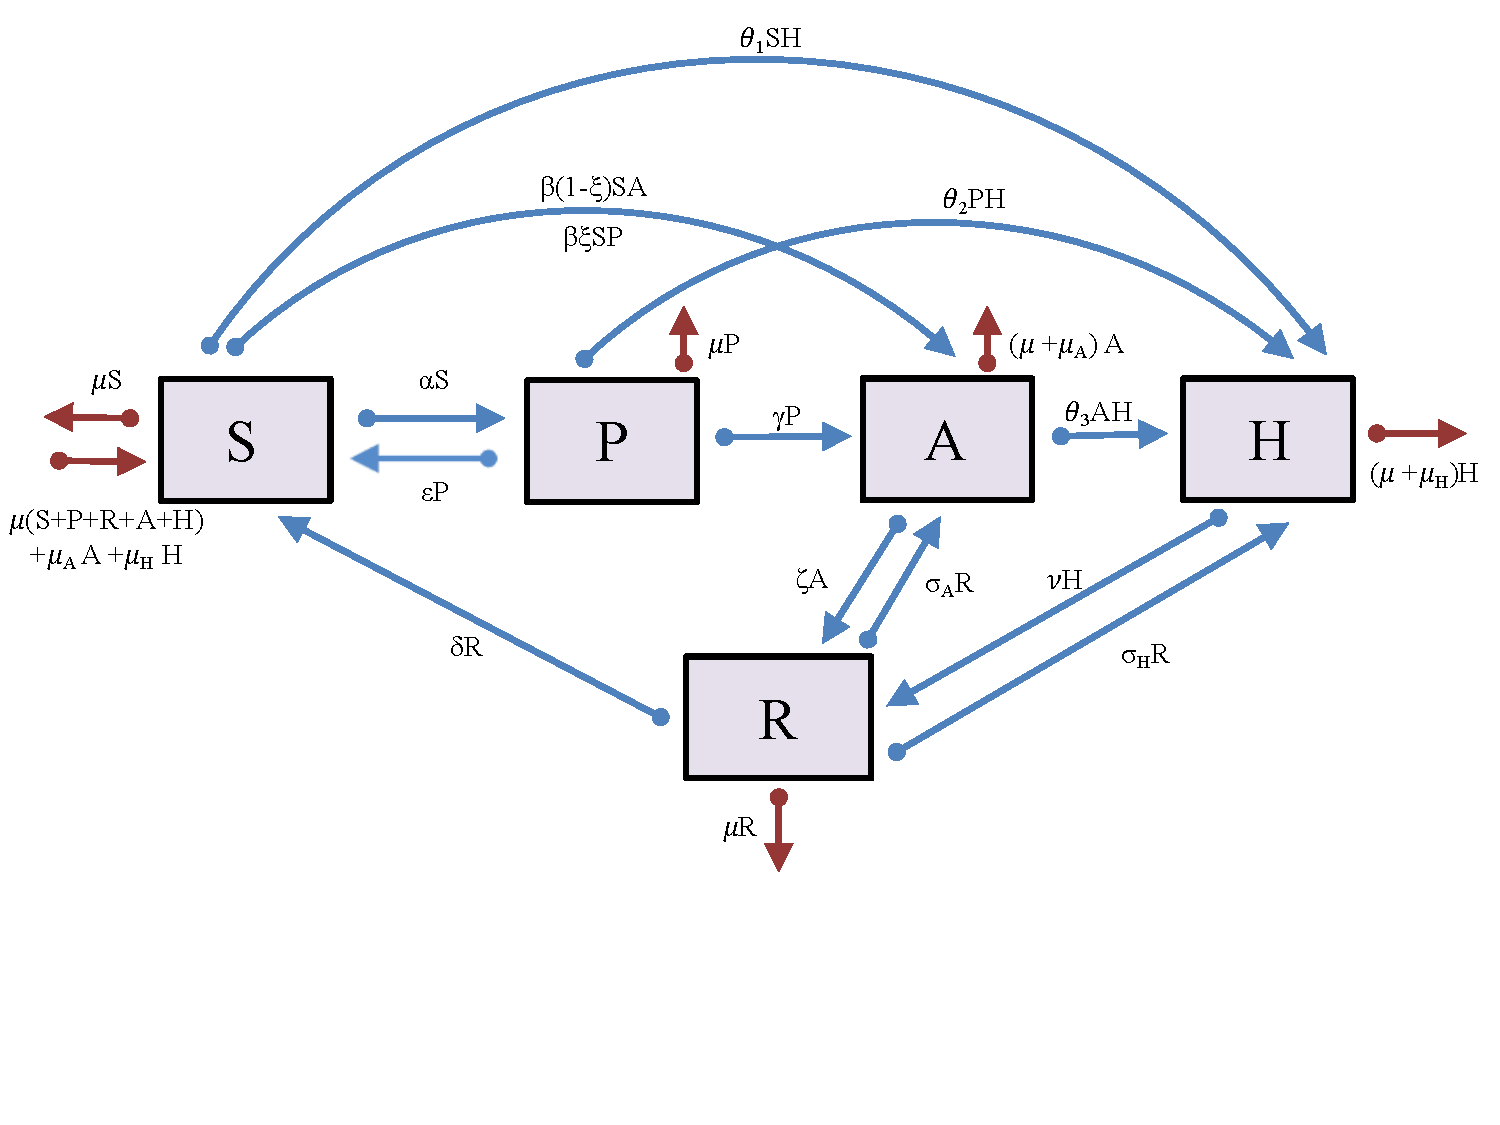
\includegraphics[height=7.5cm, width=12.8cm]{heroin_schematic.pdf} \hspace*{4.5cm}
\begin{center}
$\theta_1 SH$: rate of addiction to heroin by black market availability/ interaction with other users 
\end{center}
\end{frame}




\begin{frame}
\frametitle{}
\vspace{-.52cm}
\hspace*{-1.08cm} 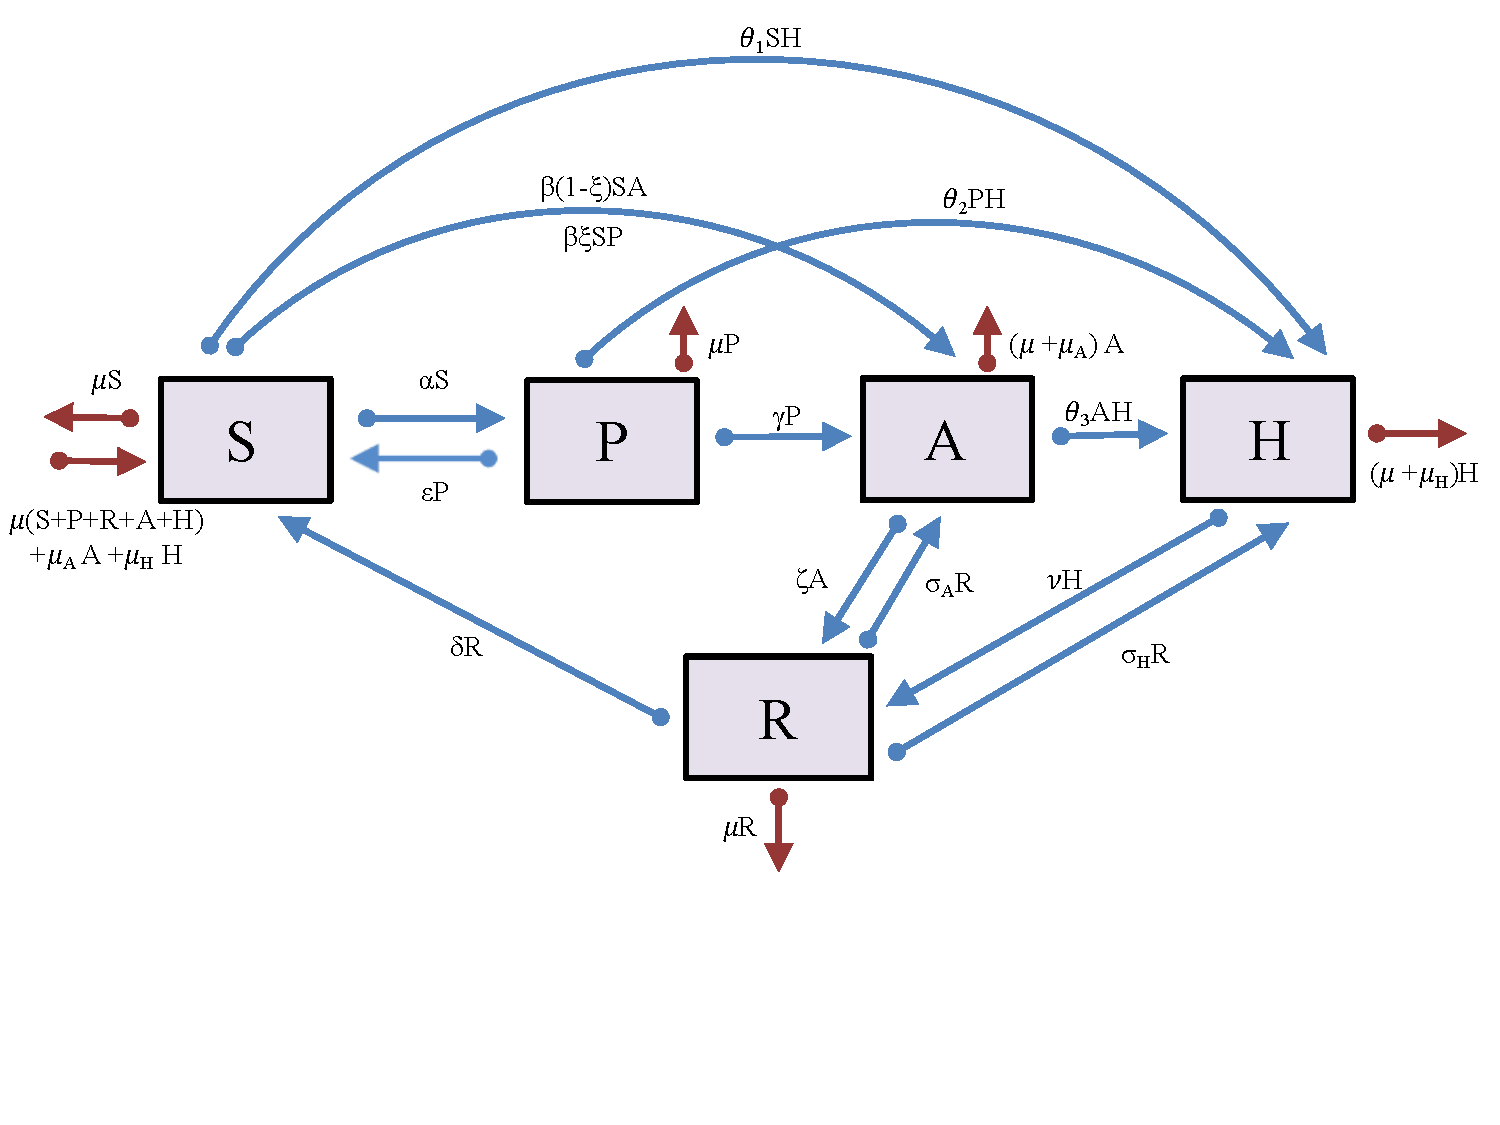
\includegraphics[height=7.5cm, width=12.8cm]{heroin_schematic.pdf} \hspace*{4.5cm}
\begin{center}
$\epsilon P$: rate of non-addicted opioid prescribed users back to susceptible
\end{center}
\end{frame}




\begin{frame}
\frametitle{}
\vspace{-.52cm}
\hspace*{-1.08cm} 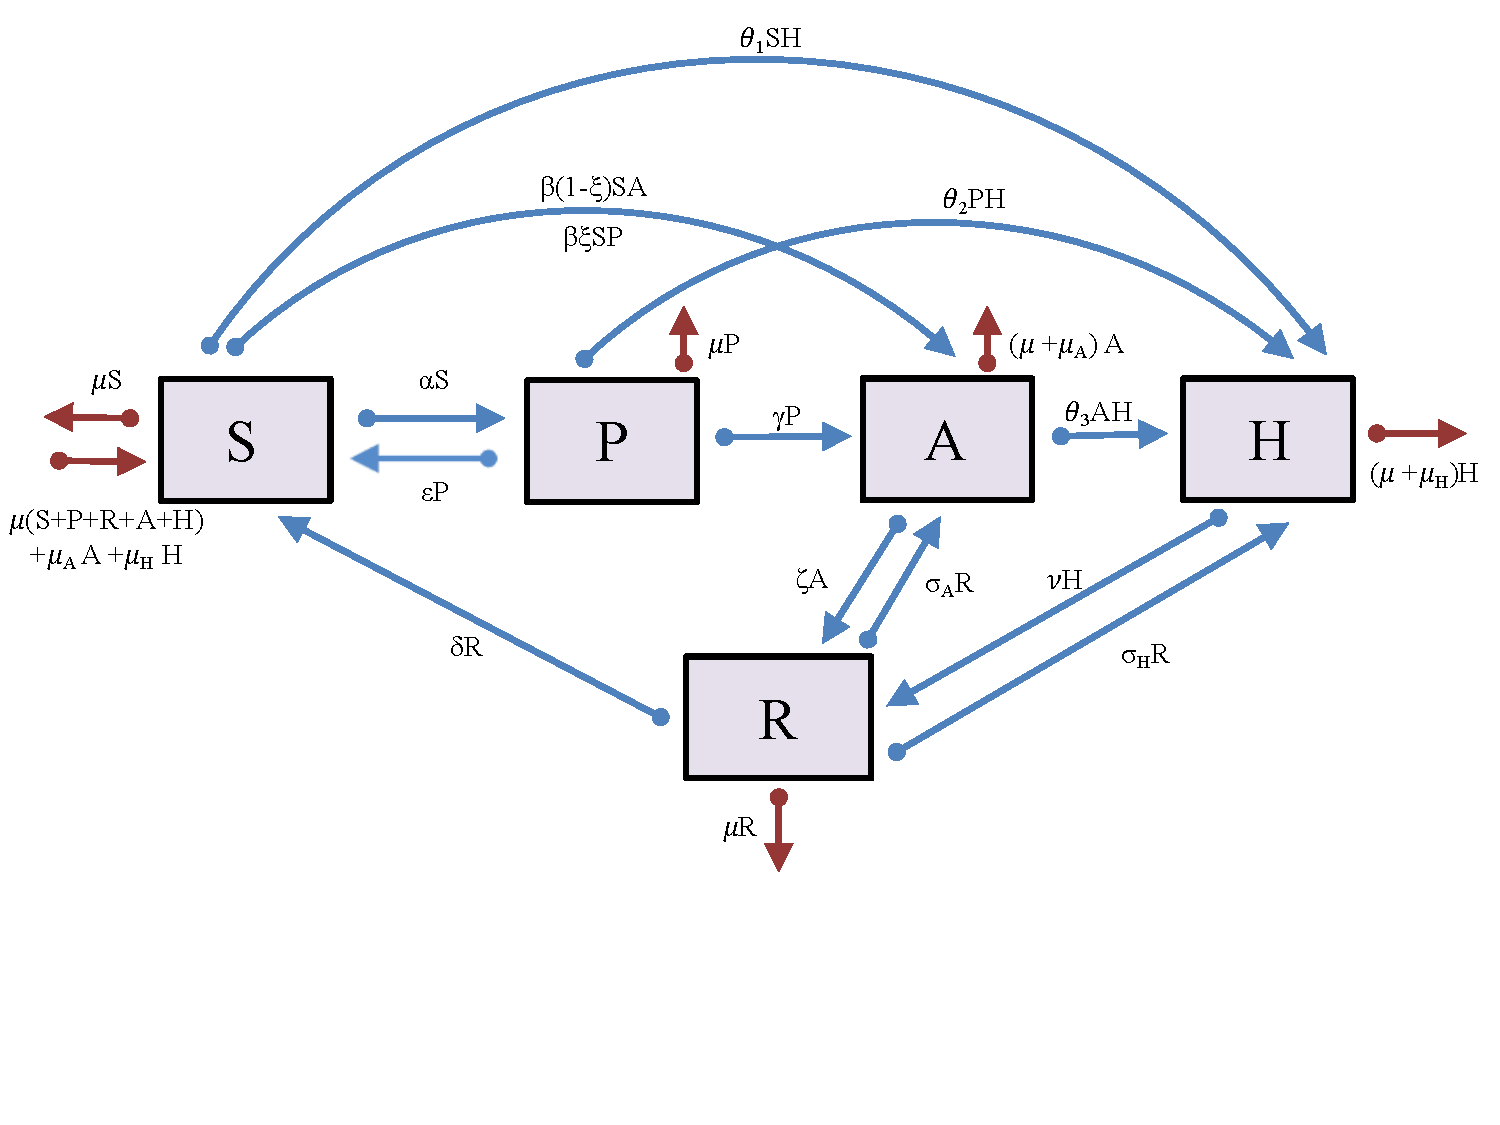
\includegraphics[height=7.5cm, width=12.8cm]{heroin_schematic.pdf} \hspace*{4.5cm}
\begin{center}
$\delta R$: rate of opioid and heroin addicts successfully finishing treatment
\end{center}
\end{frame}




\begin{frame}
\frametitle{}
\vspace{-.52cm}
\hspace*{-1.08cm} 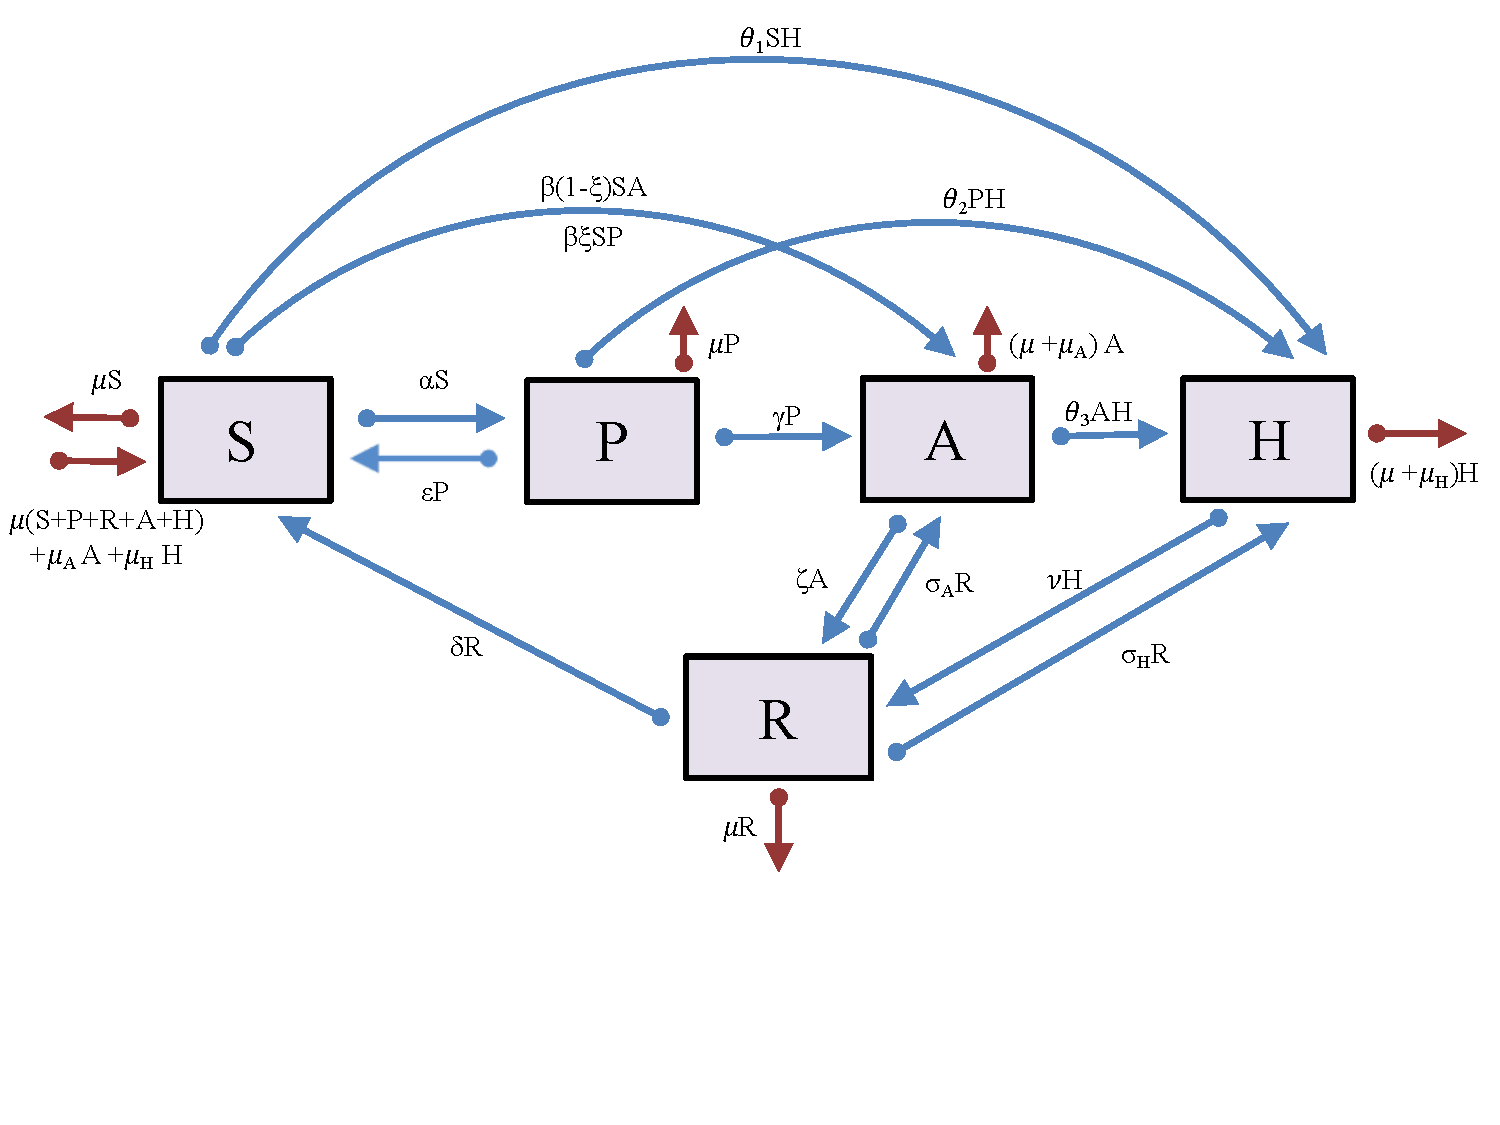
\includegraphics[height=7.5cm, width=12.8cm]{heroin_schematic.pdf} \hspace*{4.5cm}
\begin{center}
 $\mu S$, $\mu P$, $\mu A$, $\mu H$, $\mu R$: natural death rates
\end{center}
\end{frame}




\begin{frame}
\frametitle{}
\vspace{-.52cm}
\hspace*{-1.08cm} 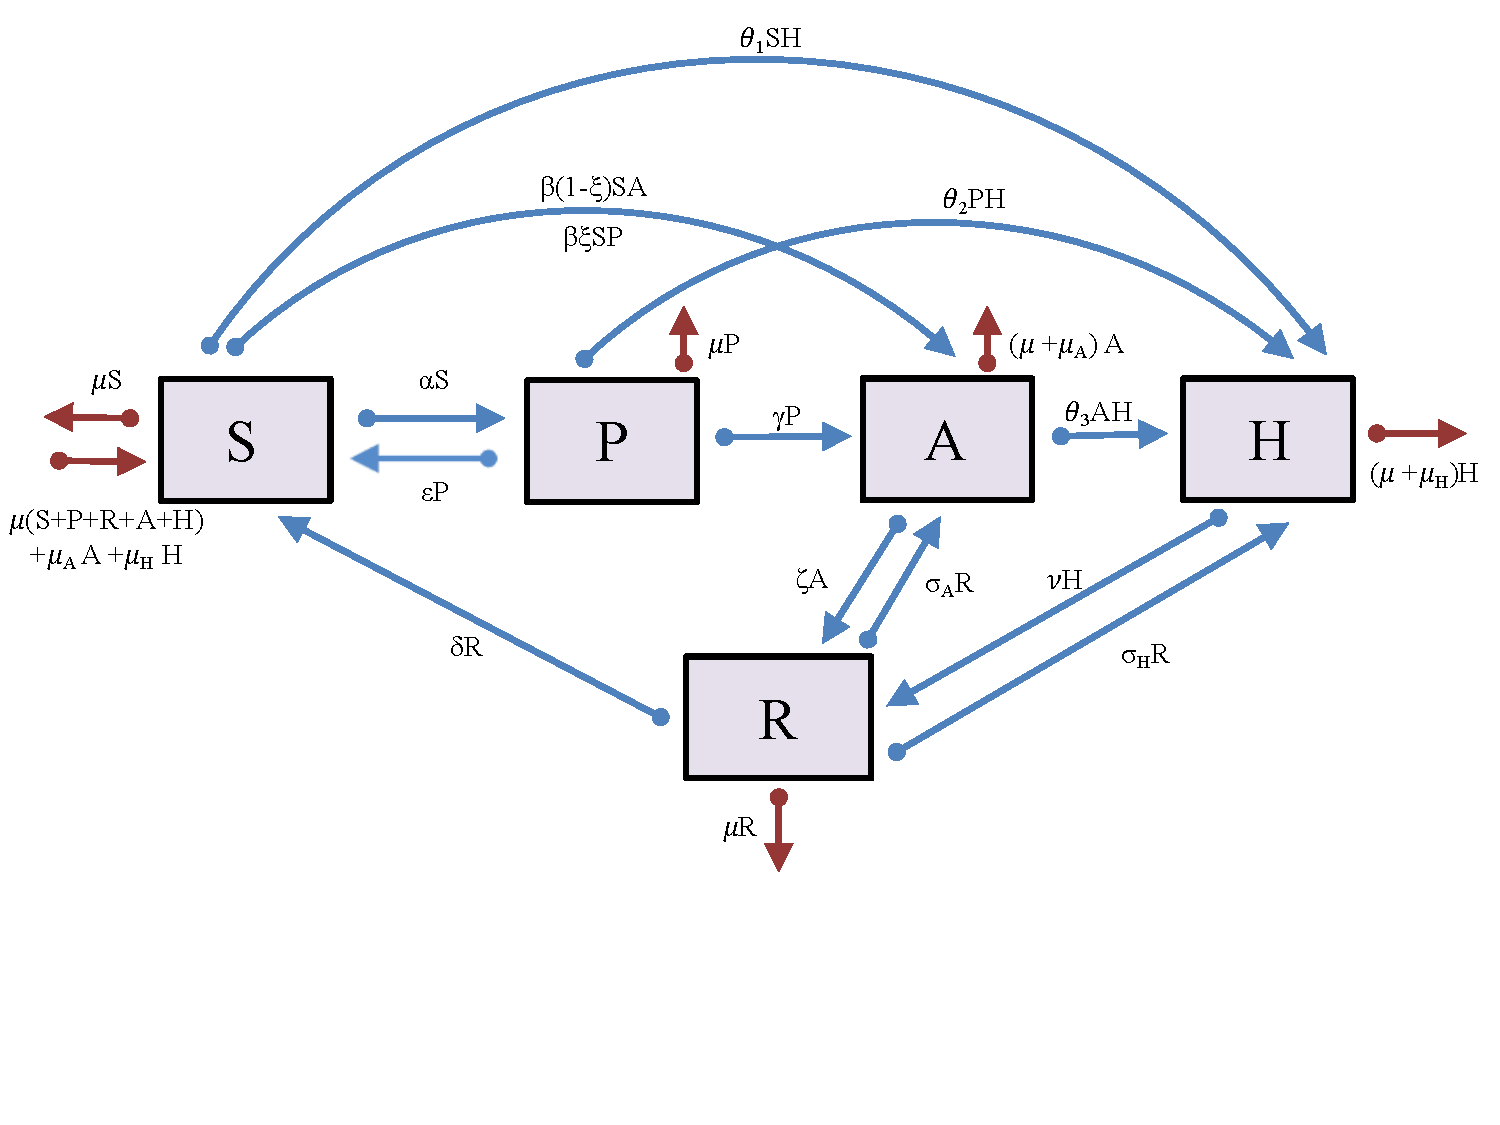
\includegraphics[height=7.5cm, width=12.8cm]{heroin_schematic.pdf} \hspace*{4.5cm}
\begin{center}
$\mu_A A$: opioid addict overdose death rate 
\end{center}
\end{frame}




\begin{frame}
\frametitle{}
\vspace{-.52cm}
\hspace*{-1.08cm} 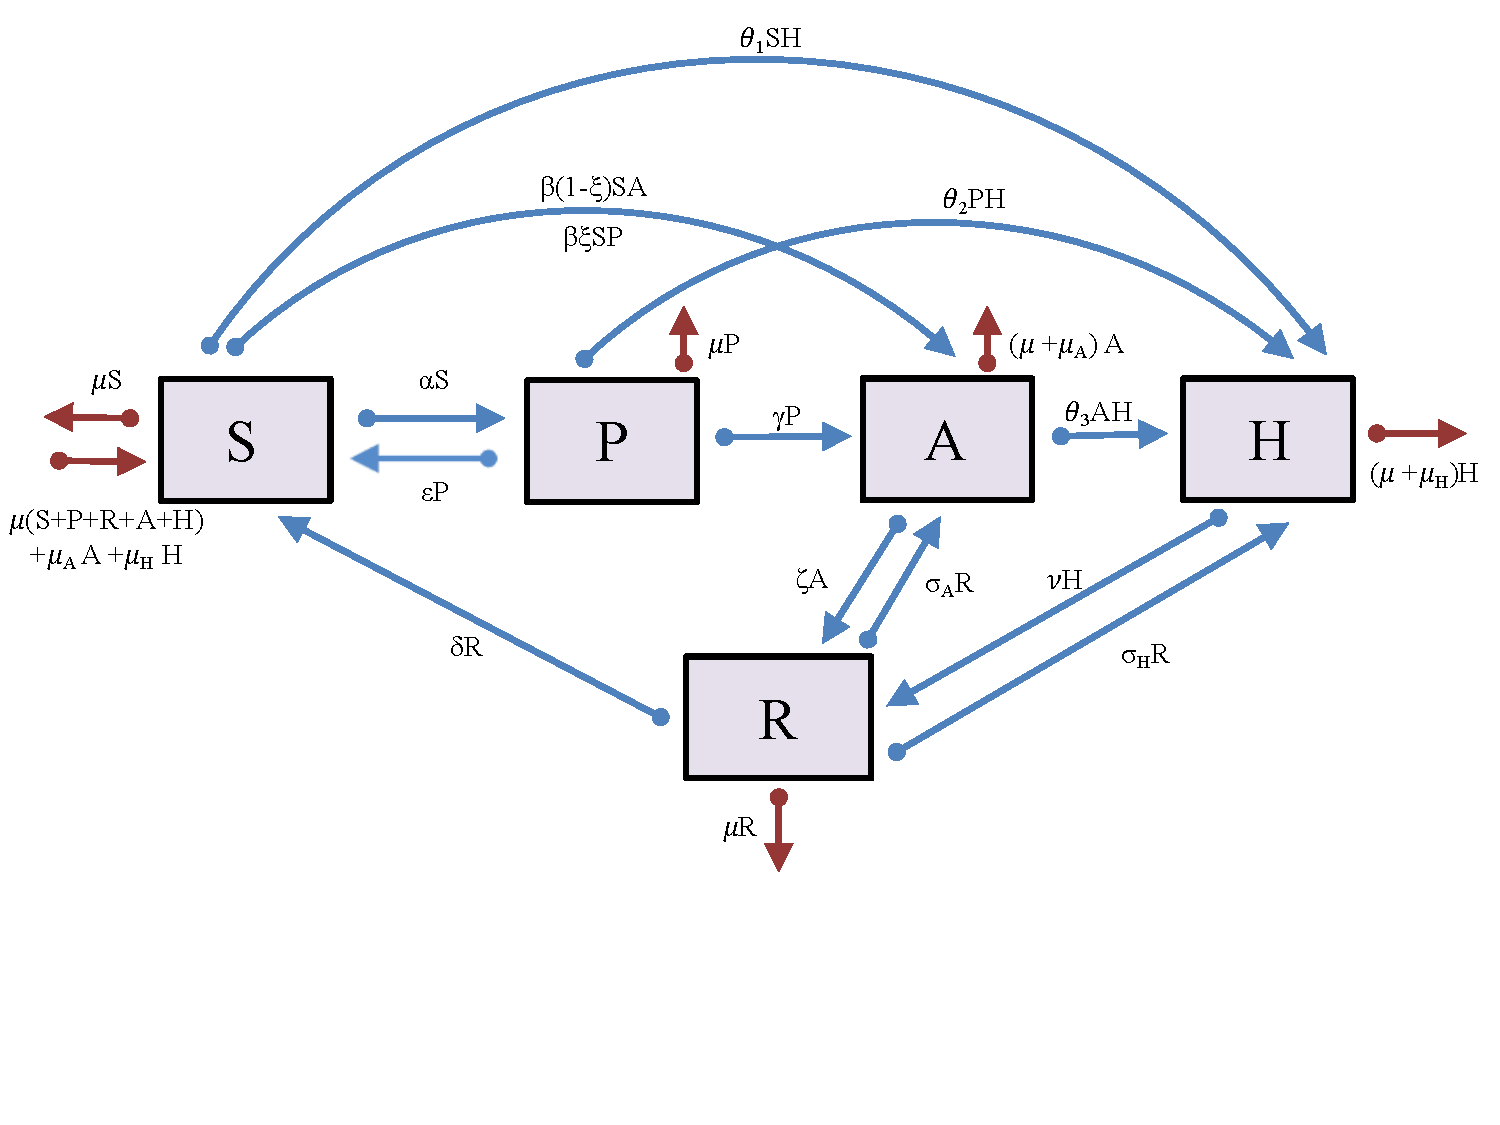
\includegraphics[height=7.5cm, width=12.8cm]{heroin_schematic.pdf} \hspace*{4.5cm}
\begin{center}
$\mu_H H$: heroin user overdose death rate 
\end{center}
\end{frame}




\begin{frame}
\frametitle{}
\vspace{-.52cm}
\hspace*{-1.08cm} 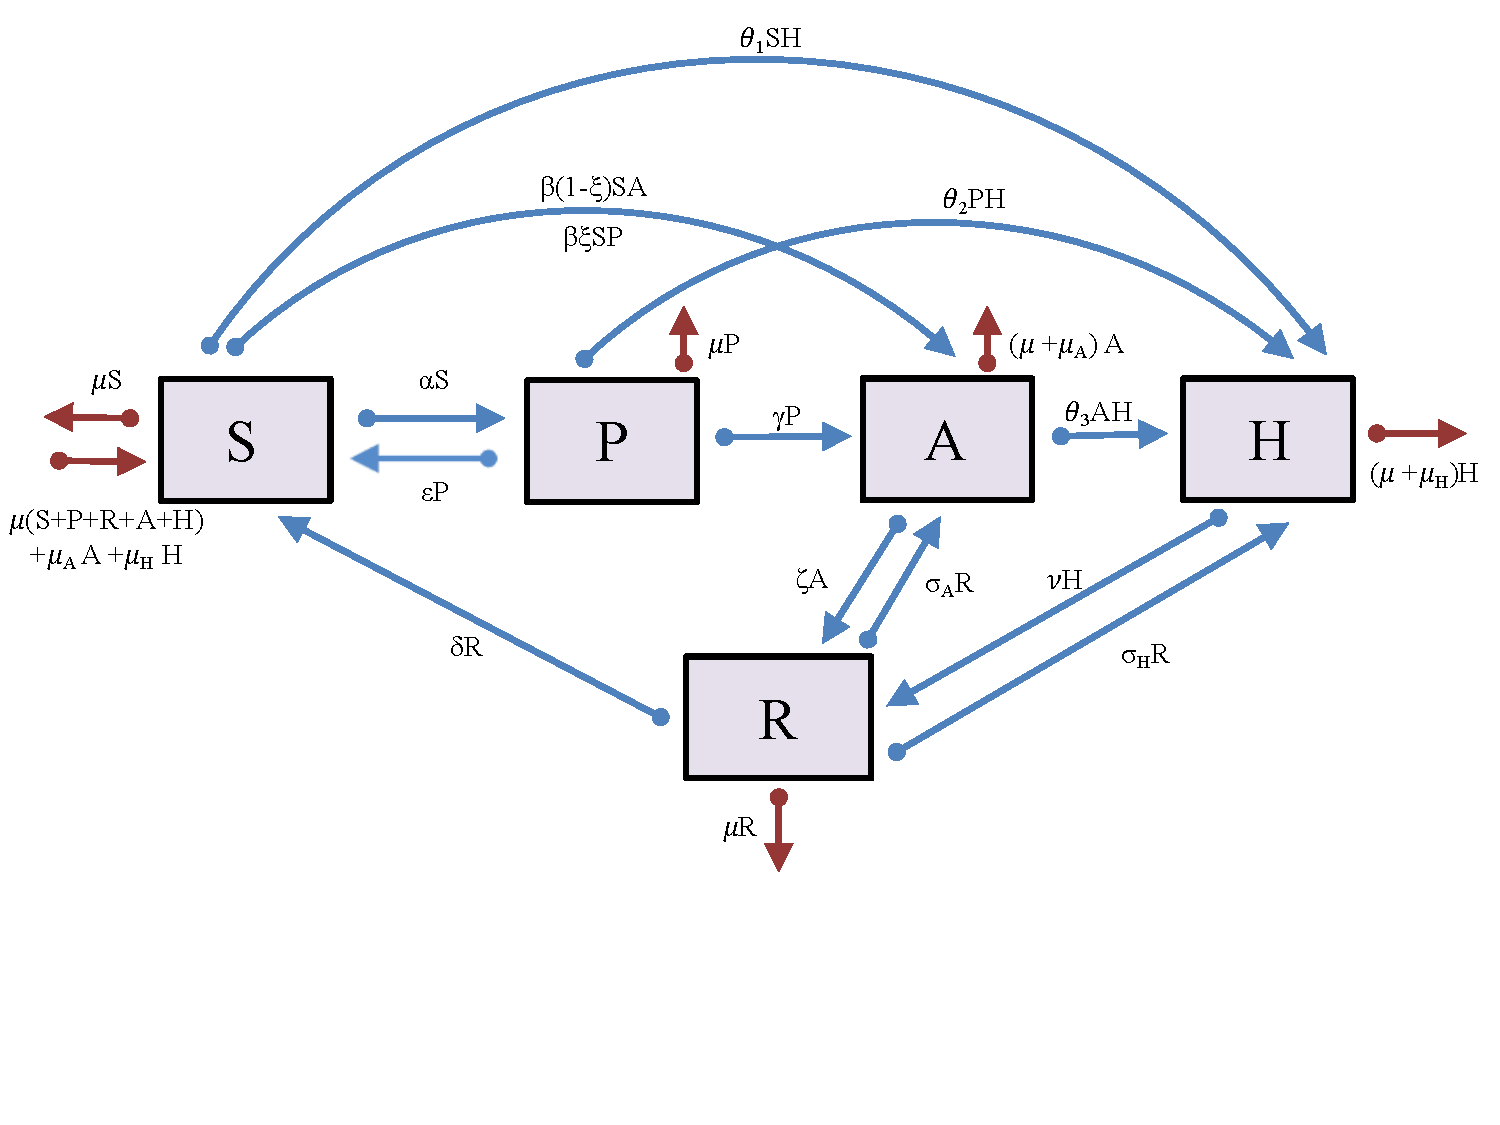
\includegraphics[height=7.5cm, width=12.8cm]{heroin_schematic.pdf} \hspace*{4.5cm}
\begin{center}
$\gamma P$: rate of opioid addiction for prescribed users
\end{center}
\end{frame}




\begin{frame}
\frametitle{}
\vspace{-.52cm}
\hspace*{-1.08cm} 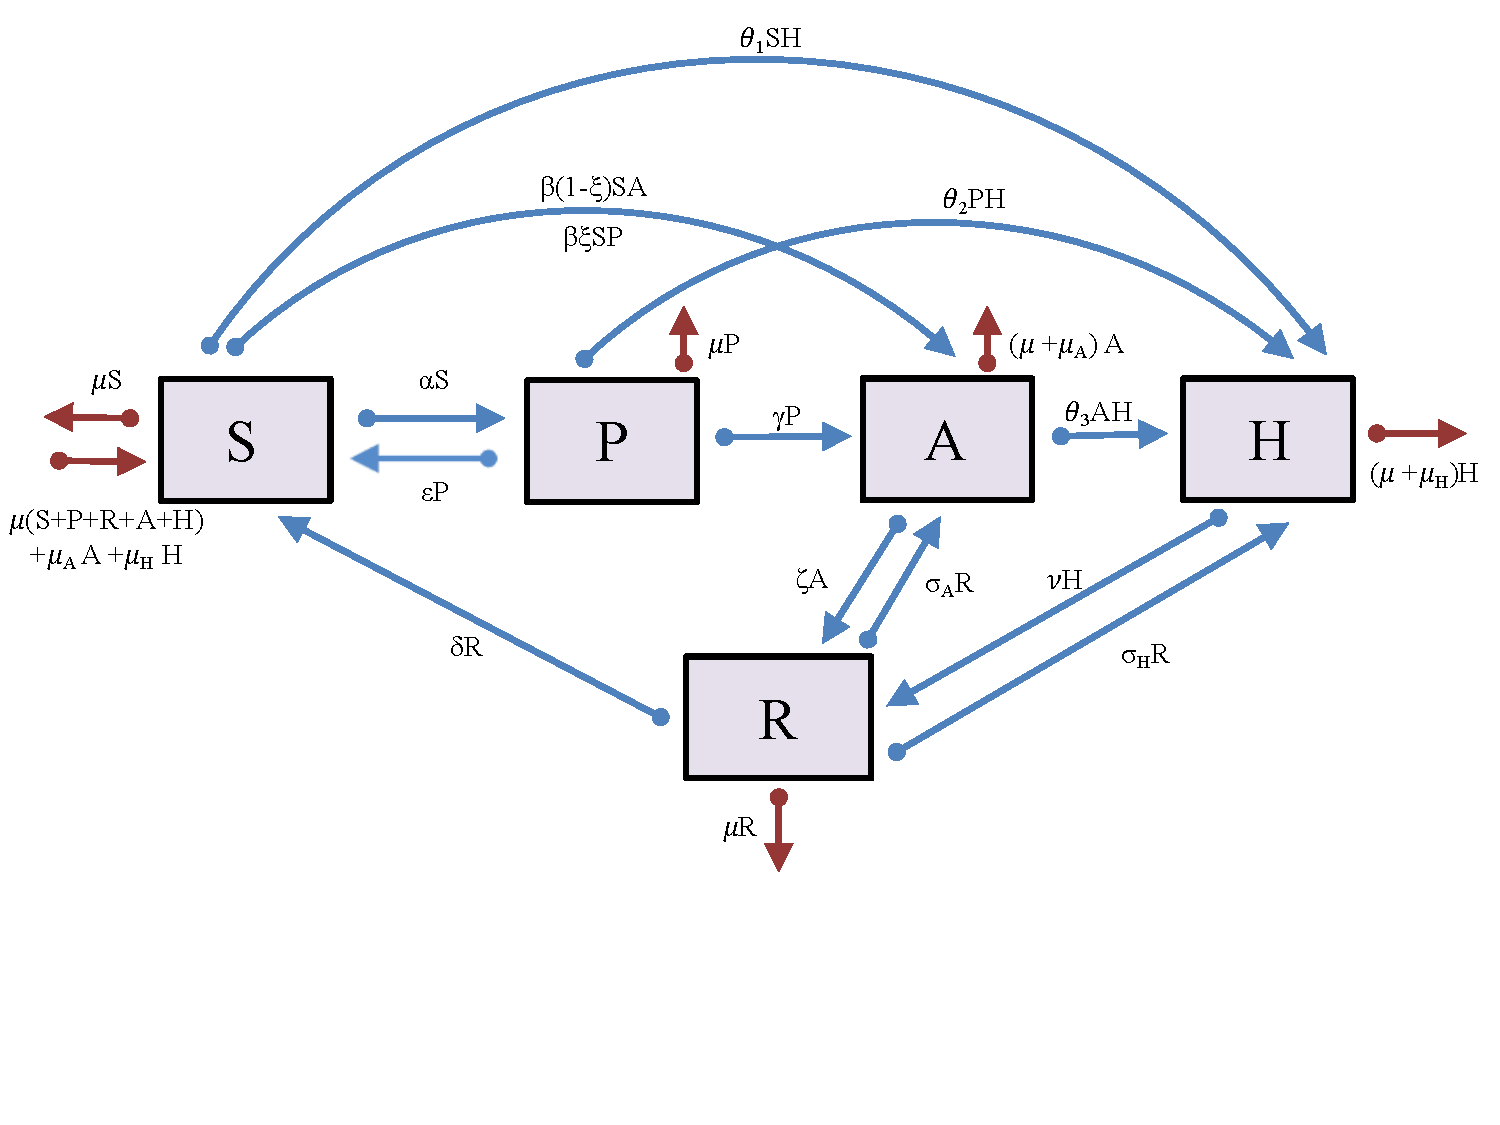
\includegraphics[height=7.5cm, width=12.8cm]{heroin_schematic.pdf} \hspace*{4.5cm}\begin{center}
$\theta_2 PH$: rate of heroin addiction for prescribed users 
\end{center}
\end{frame}



\begin{frame}
\frametitle{}
\vspace{-.52cm}
\hspace*{-1.08cm} 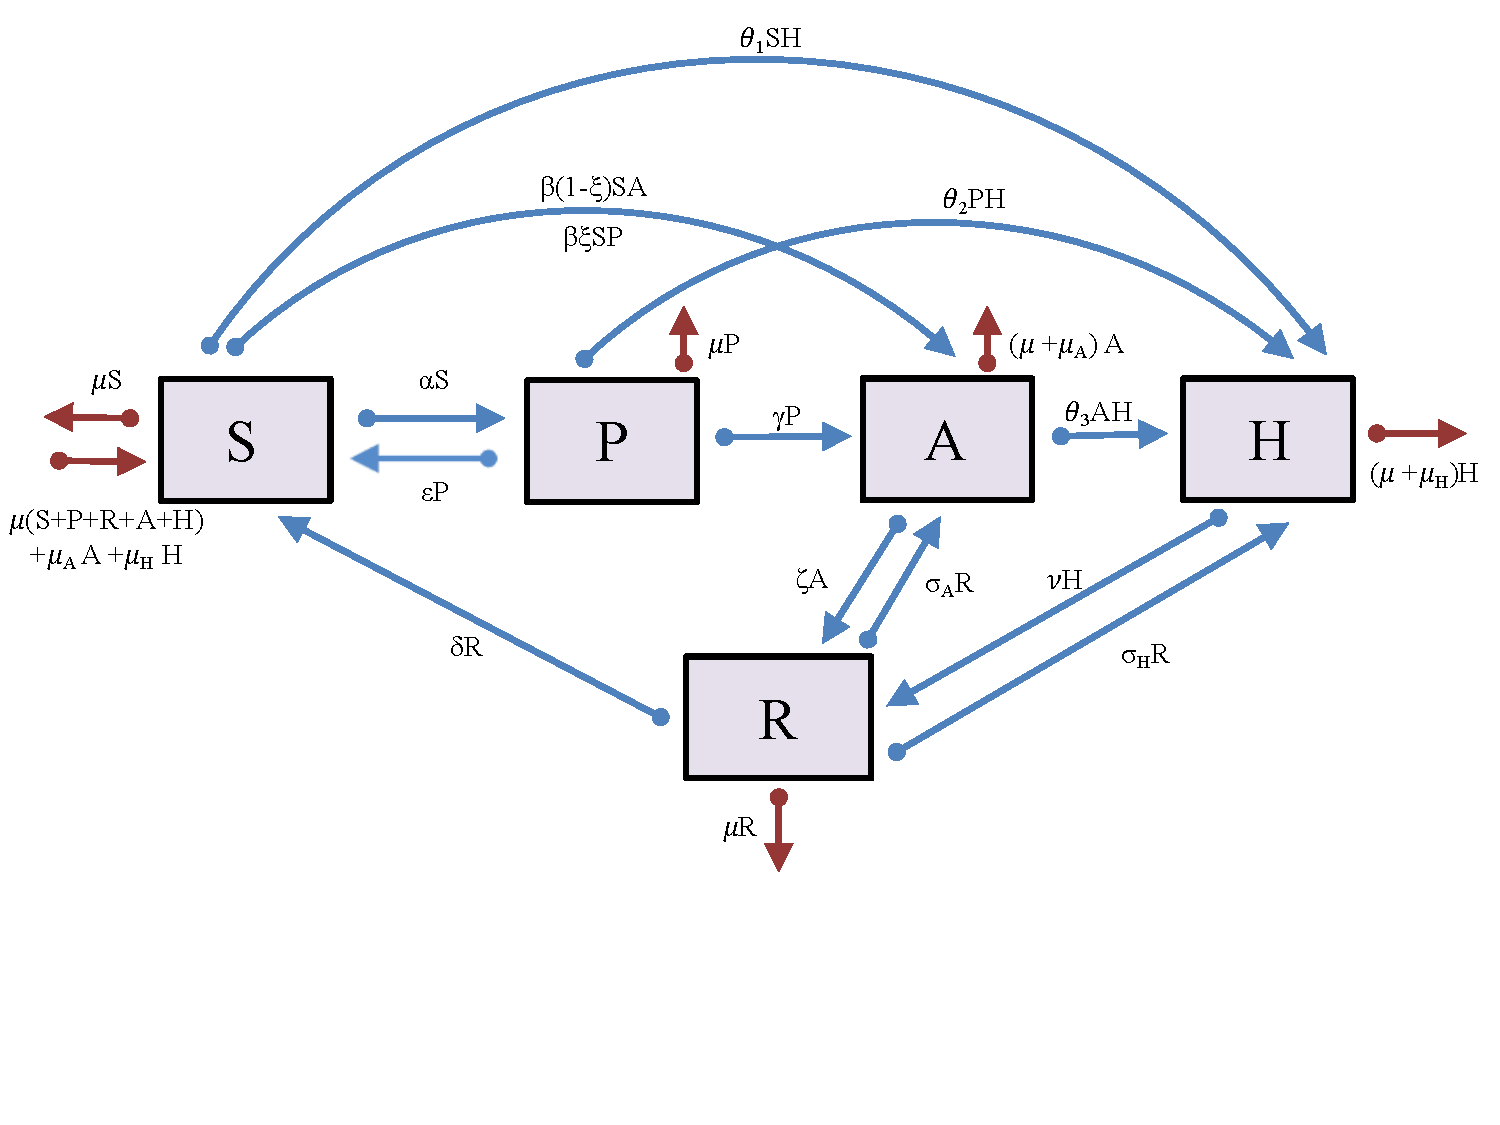
\includegraphics[height=7.5cm, width=12.8cm]{heroin_schematic.pdf} \hspace*{4.5cm}
\begin{center}
$\zeta A$: rate addicted opioid users enter treatment
\end{center}
\end{frame}




\begin{frame}
\frametitle{}
\vspace{-.56cm}
\hspace*{-1.08cm} 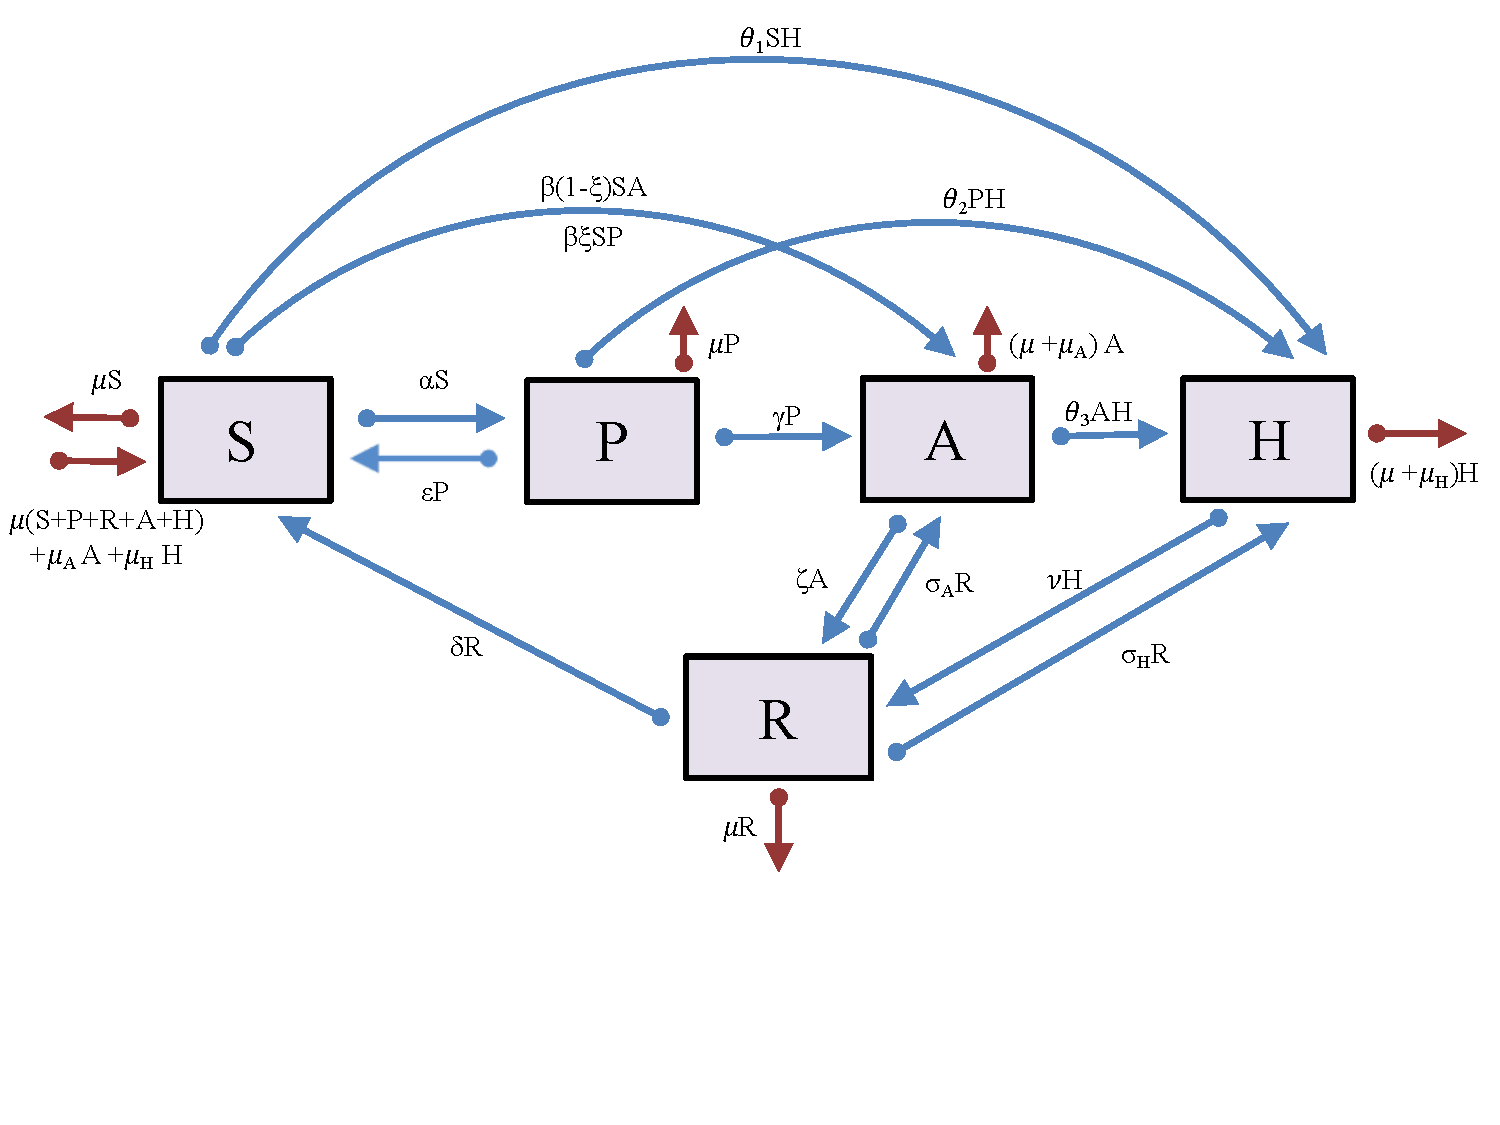
\includegraphics[height=7.5cm, width=12.8cm]{heroin_schematic.pdf} \hspace*{4.5cm}
\begin{center}
$\nu H$: rate heroin users enter treatment 
\end{center}
\end{frame}


\begin{frame}
\frametitle{}
\vspace{-.52cm}
\hspace*{-1.08cm} 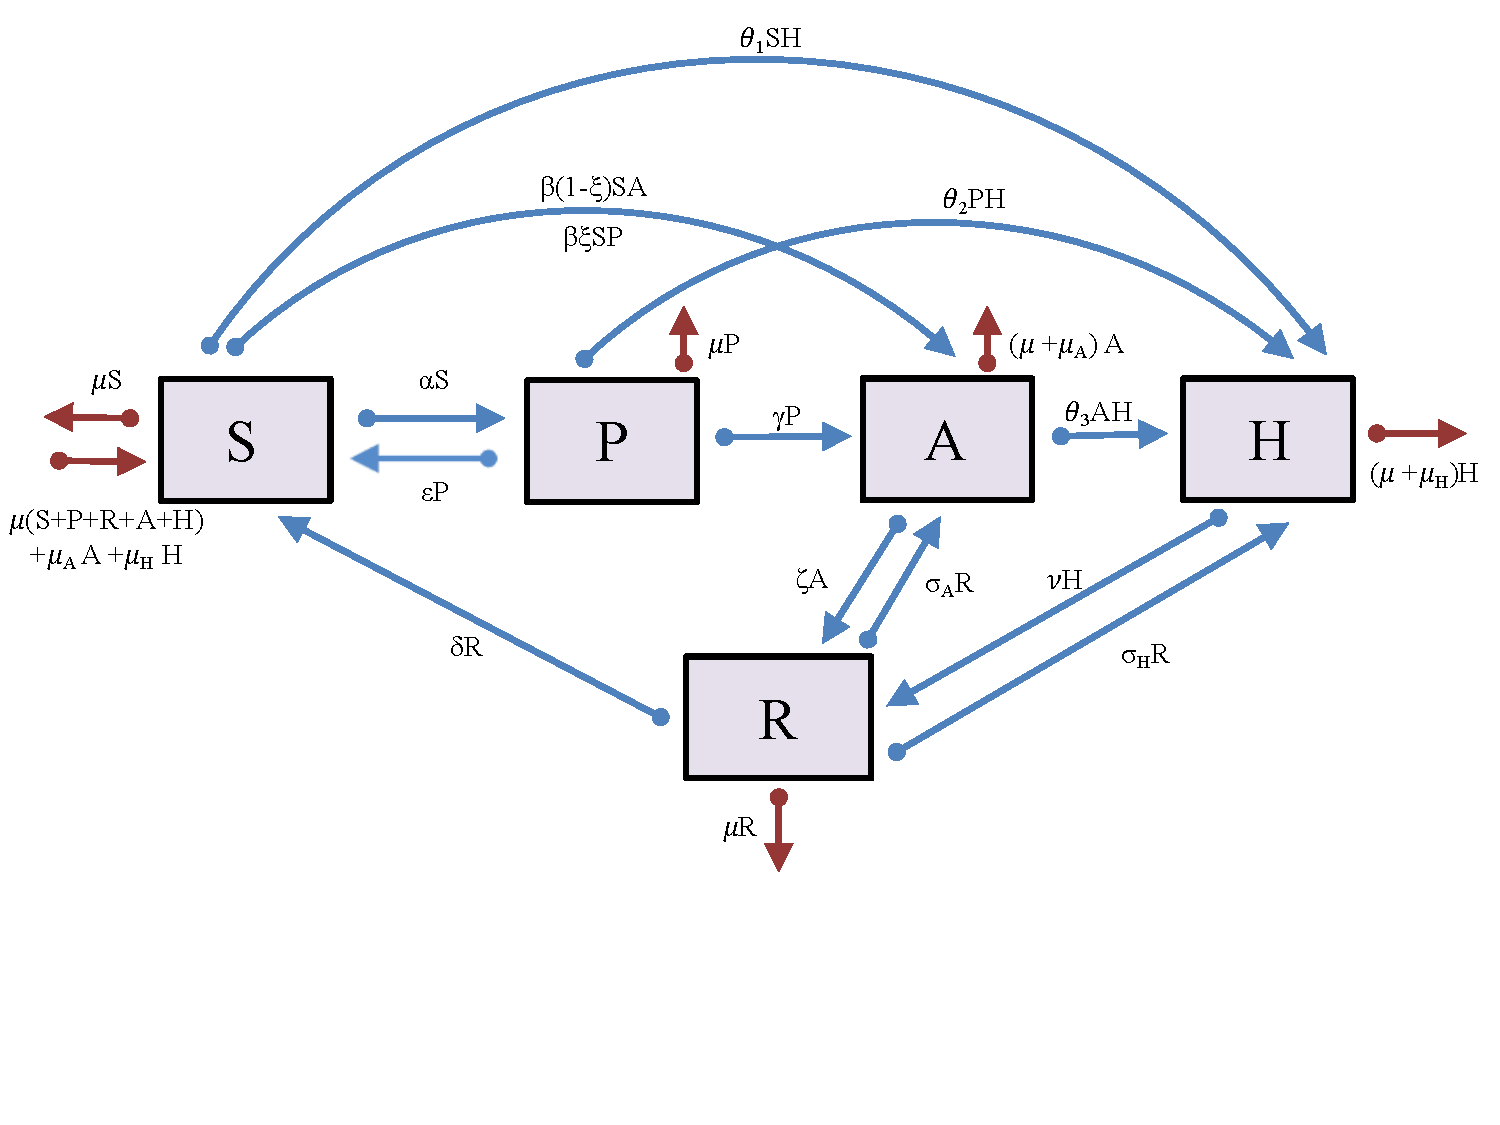
\includegraphics[height=7.5cm, width=12.8cm]{heroin_schematic.pdf} \hspace*{4.5cm}\begin{center}
$\sigma_A R$: transition rate from treatment into the opioid addicted class  
\end{center}
\end{frame}




\begin{frame}
\frametitle{}
\vspace{-.52cm}
\hspace*{-1.08cm} 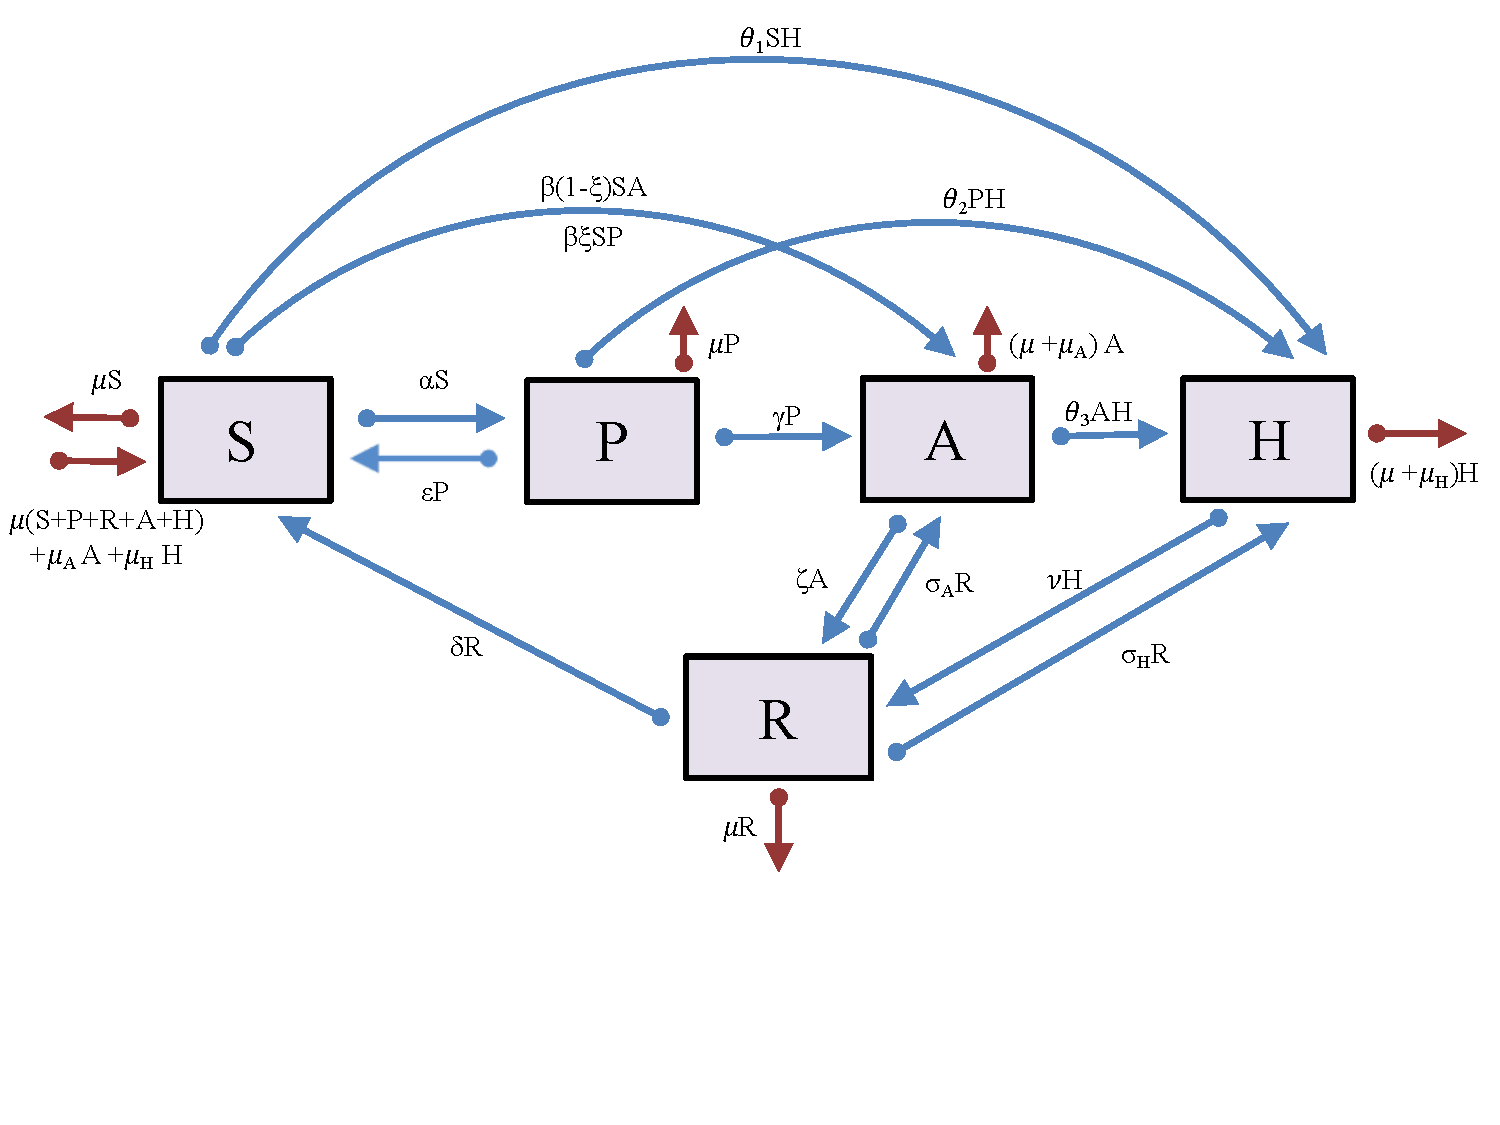
\includegraphics[height=7.5cm, width=12.8cm]{heroin_schematic.pdf} \hspace*{4.5cm}
\begin{center}
$\sigma_H R$: transition rate from treatment into the heroin addicted class 
\end{center}
\end{frame}





\begin{frame}
\frametitle{}
\vspace{-.52cm}
\hspace*{-1.08cm} 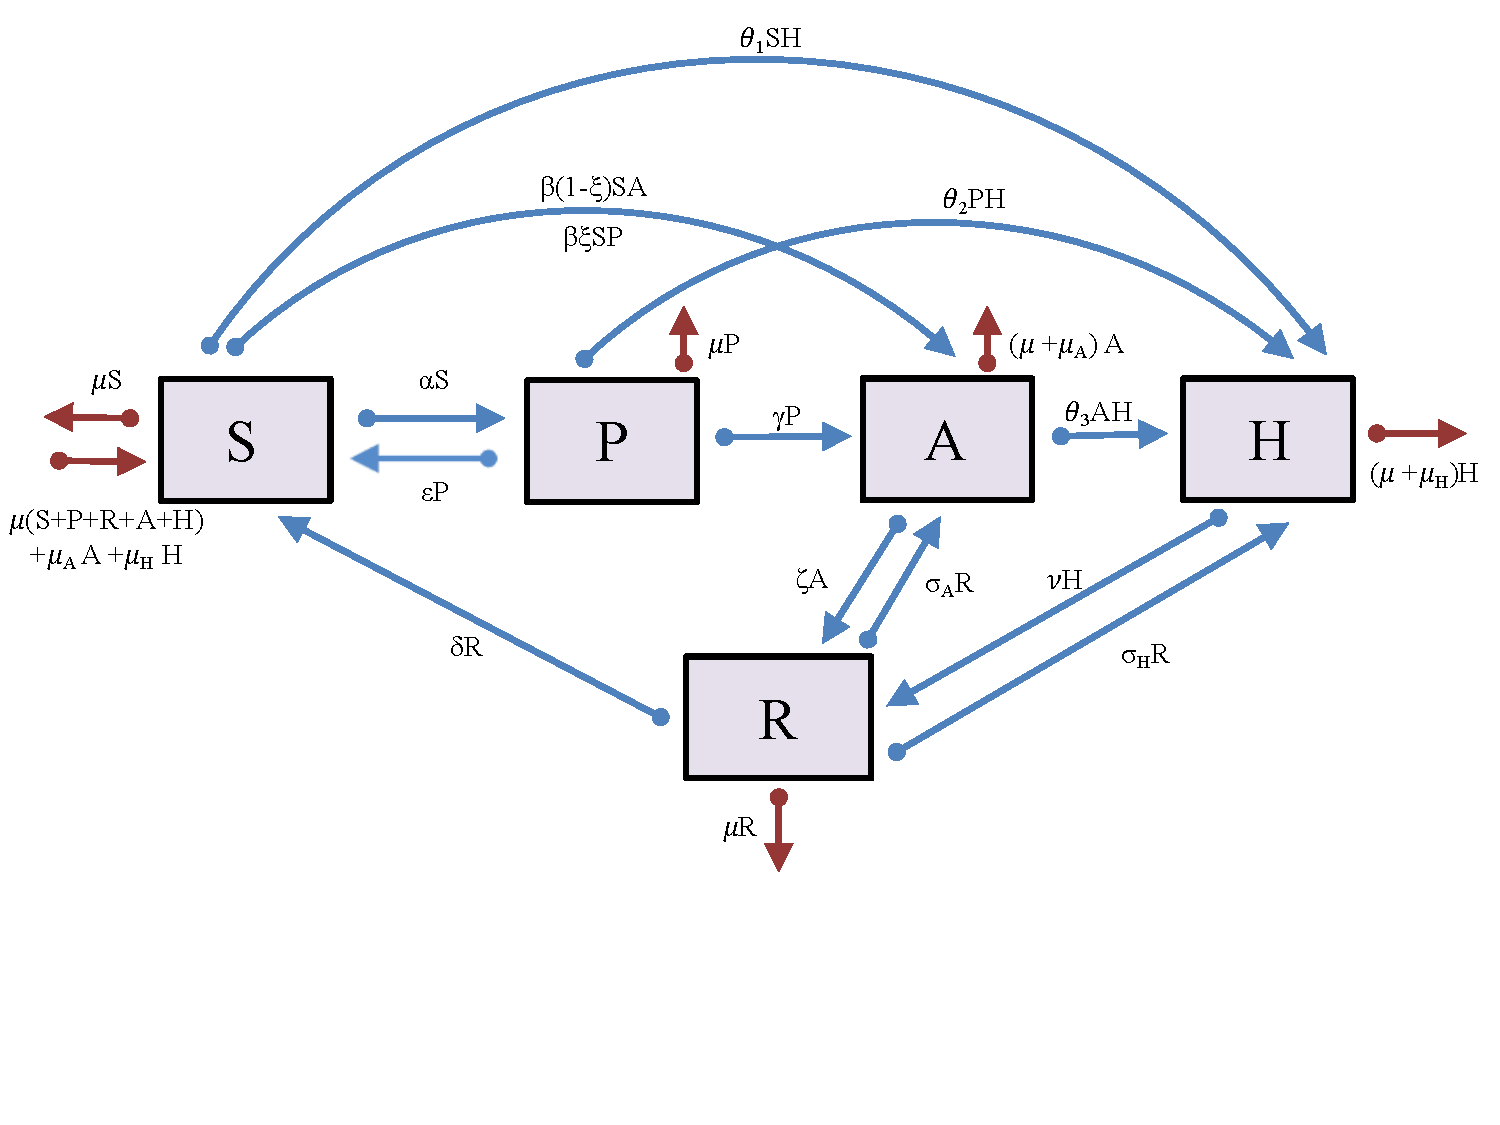
\includegraphics[height=7.5cm, width=12.8cm]{heroin_schematic.pdf} \hspace*{4.5cm}
\begin{center}
$\theta_3 AH$: heroin addiction rate from opioid addicted 
\end{center}
\end{frame}







\begin{comment}
\begin{frame}
\frametitle{Model Formulation}
\begin{columns}
\begin{column}{0.5\textwidth} 
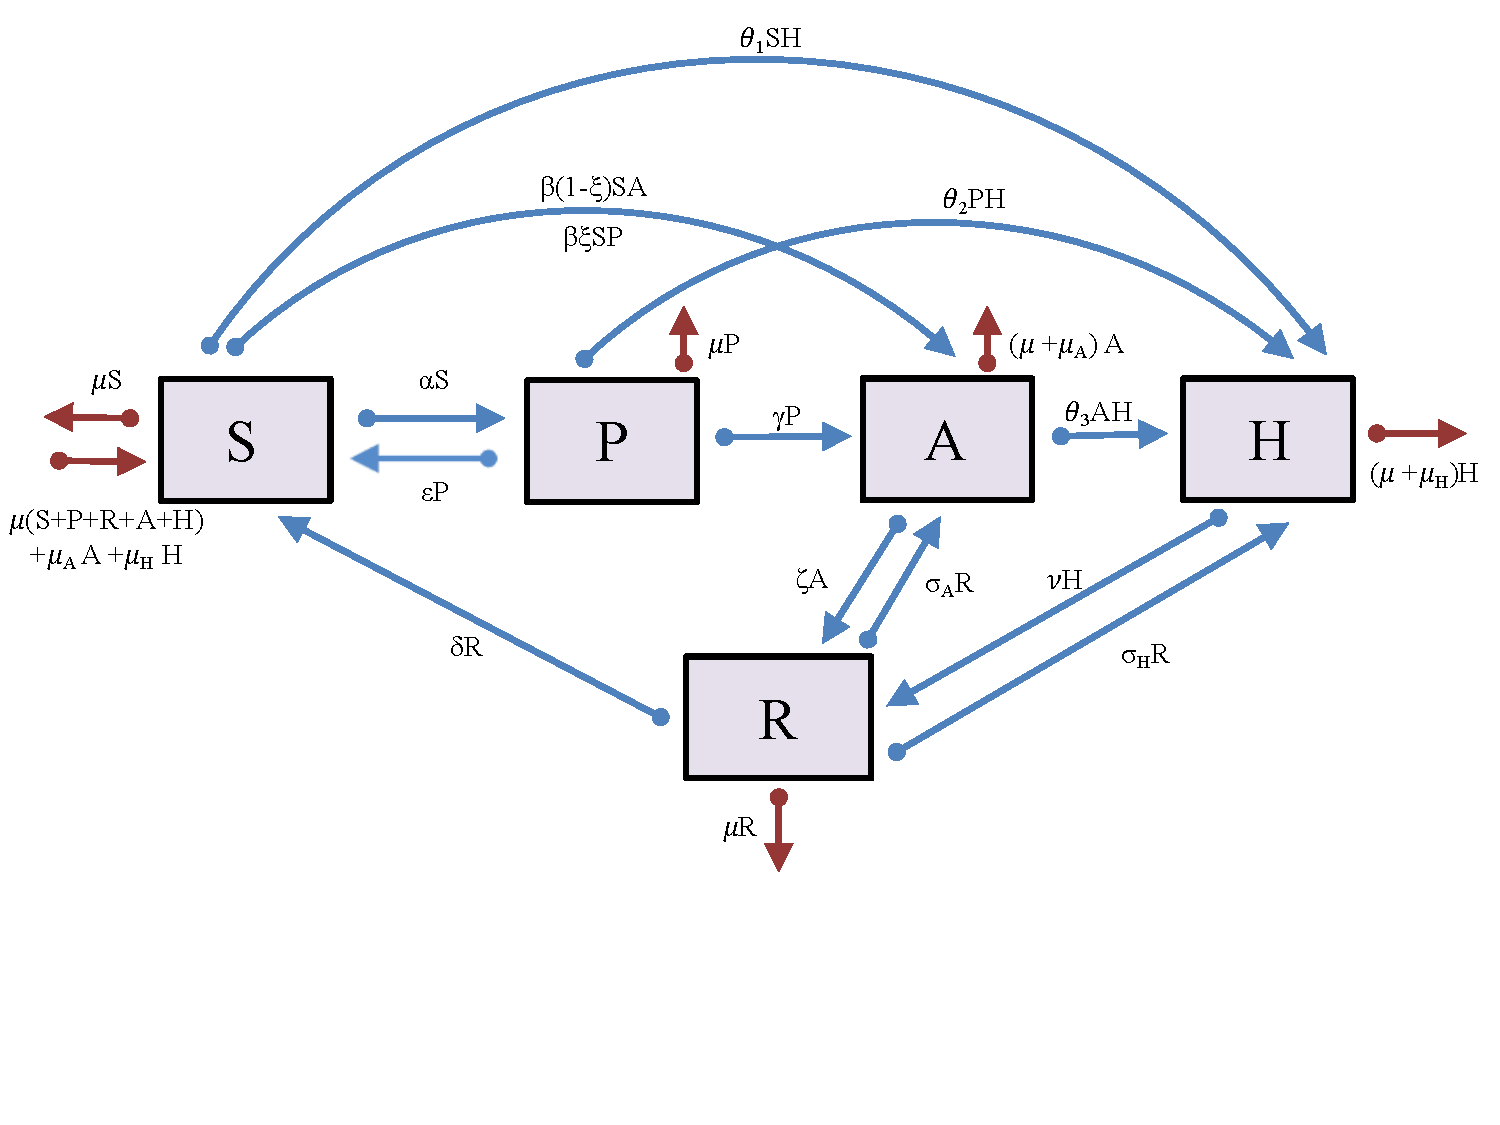
\includegraphics[height=4cm, width=7cm]{heroin_schematic.pdf}
\end{column}
\begin{column}{0.5\textwidth}
\begin{itemize}
\vspace{-0.2cm} 
\item<1>Parameters:
\begin{enumerate}[-]
\item<1> $\alpha S$: prescription rate 
%\item<1> $\beta$ : total probability of opioid addiction by non-prescription means
\item<1> $\beta(1-\xi)SA$: opioid addiction rate by black market drugs/interaction with other addicts 
\item<1>  $\beta \xi SP$ : opioid addiction rate by obtaining extra prescription opioids 
\end{enumerate}
\end{itemize}
\end{column}
\end{columns}
\end{frame}
\end{comment}

\begin{comment}
\begin{frame}
\frametitle{Model Formulation}
\begin{columns}
\begin{column}{0.5\textwidth} 
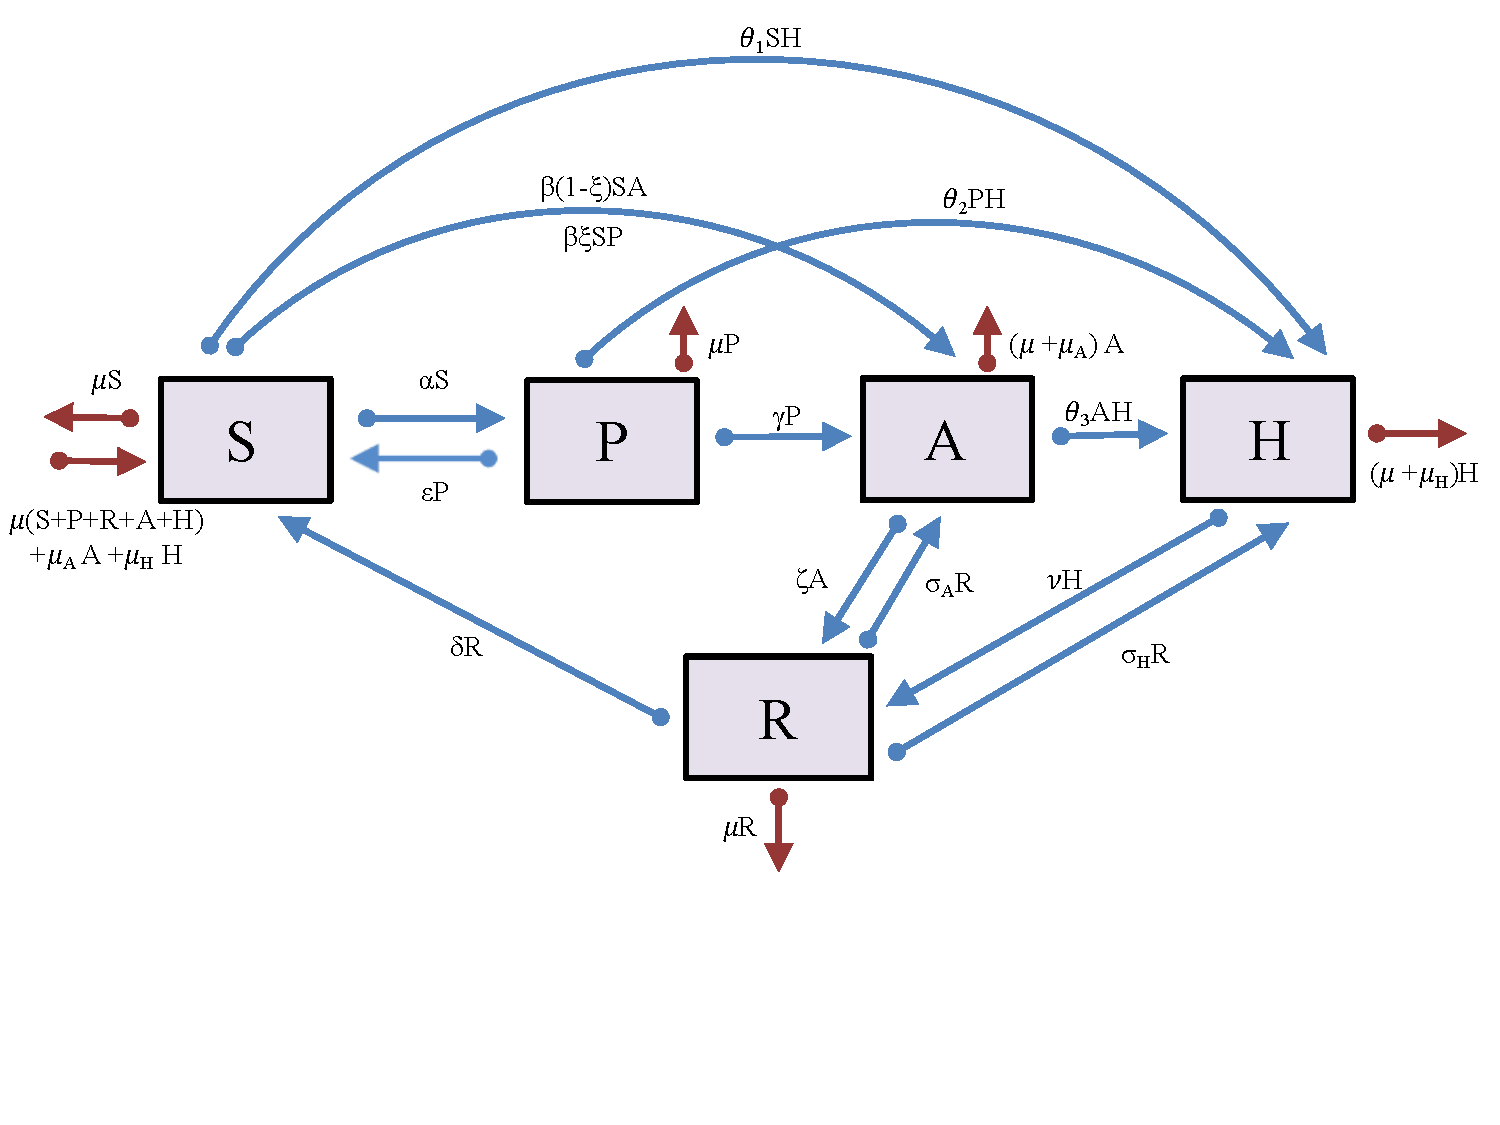
\includegraphics[height=4cm, width=7cm]{heroin_schematic.pdf}
\end{column}
\begin{column}{0.5\textwidth}
\vspace{-0.6cm} 
\begin{itemize}
\item<1>Parameters:
\begin{enumerate}[-]
\vspace{.1cm}
\item<1> $\theta_1 SH$: rate of addiction to heroin by black market availability/ interaction with other users 
\vspace{.1cm}
\item<1>$\epsilon P$: rate of non-addicted opioid prescribed users back to susceptible
\vspace{.1cm} 
\item<1>$\delta R$: rate of opioid and heroin addicts successfully finishing treatment
\end{enumerate}
\end{itemize}
\end{column}
\end{columns}
\end{frame}
\end{comment}


\begin{comment}
\begin{frame}
\frametitle{Model Formulation}
\begin{columns}
\begin{column}{0.5\textwidth} 
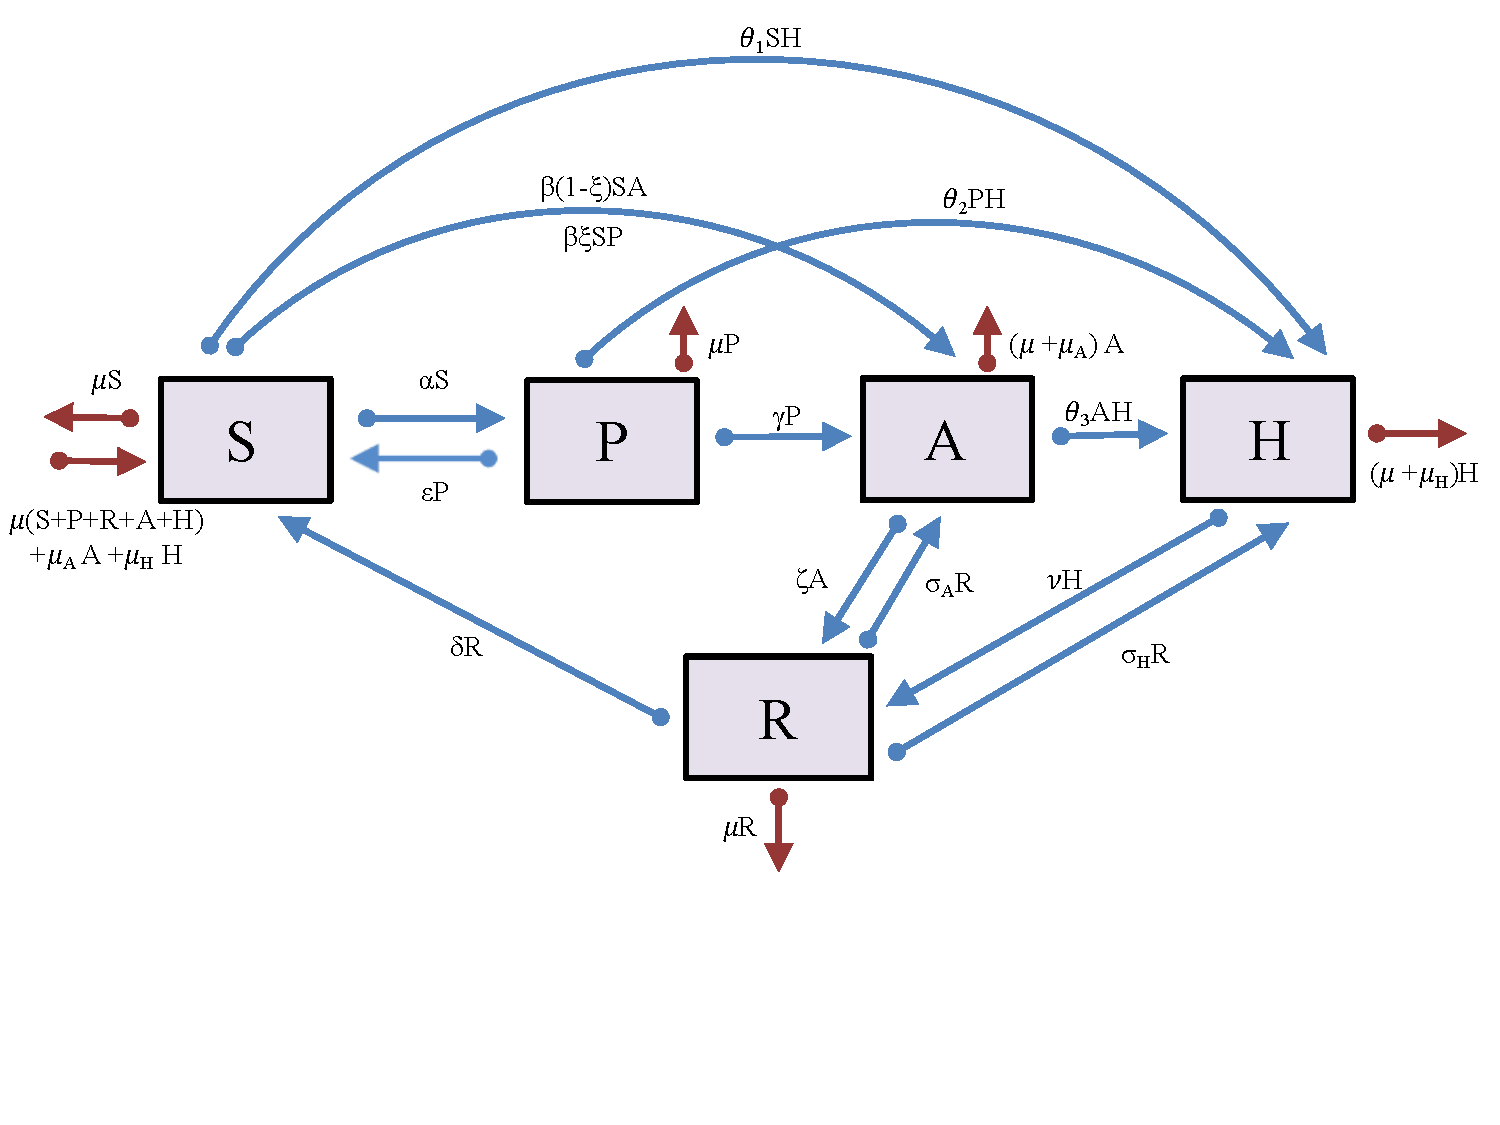
\includegraphics[height=4cm, width=7cm]{heroin_schematic.pdf}
\end{column}
\begin{column}{0.5\textwidth}

\vspace{-0.7cm} 
\begin{itemize}
 \item<1> Parameters:
\begin{enumerate}[-]
\item<1>  $\mu S$, $\mu P$, $\mu A$, $\mu H$, $\mu R$: natural death rates
\vspace{.1cm} 
\item<1> $\mu_A A$: opioid addict overdose death rate 
\vspace{.1cm} 
\item<1> $\mu_H H$: heroin user overdose death rate 
\vspace{.1cm} 
\item<1>$\gamma P$: rate of opioid addiction for prescribed users
\vspace{.1cm} 
\item<1> $\theta_2 PH$: rate of heroin addiction for prescribed users 
\end{enumerate}
\end{itemize}
\end{column}
\end{columns}
\end{frame}
\end{comment}

\begin{comment}
\begin{frame}
\frametitle{Model Formulation}
\begin{columns}
\begin{column}{0.5\textwidth} 
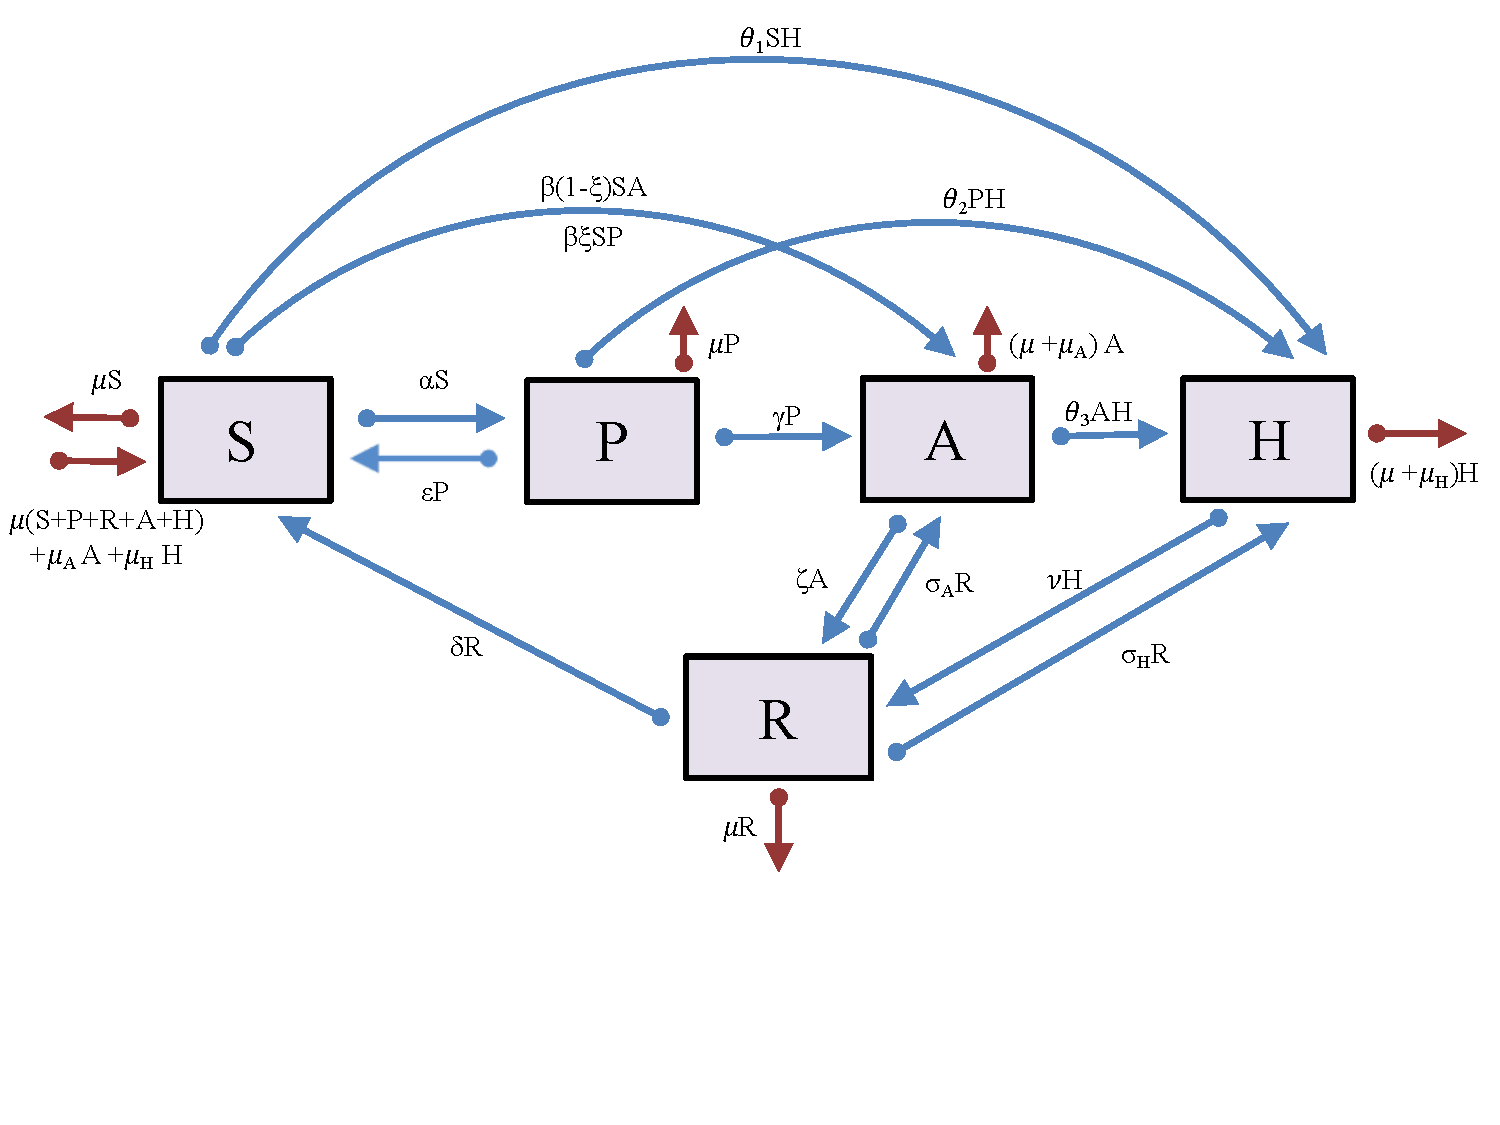
\includegraphics[height=4cm, width=7cm]{heroin_schematic.pdf}
\end{column}
\begin{column}{0.5\textwidth}
\begin{itemize}
\item<1>Parameters:
\begin{enumerate}[-]
\vspace{.2cm}
\item<1> $\sigma_A R$: transition rate from treatment into the opioid addicted class  
\item<1>  $\sigma_H R$: transition rate from treatment into the heroin addicted class 
\item<1> $\zeta A$: rate addicted opioid users enter treatment
\item<1>$\nu H$: rate heroin users enter treatment 
\item<1> $\theta_3 AH$: heroin addiction rate from opioid addicted 
\end{enumerate}
\end{itemize}
\end{column}
\end{columns}
\end{frame}
\end{comment}



\begin{frame}{System of ODEs Model}

\small

$$\dfrac{dS}{dt} = -\alpha S - \beta (1- \xi) SA  -\beta \xi SP- \theta_{1} SH +\epsilon P +\delta R + 
\mu (P+R) + (\mu+\mu_{A})A + (\mu+\mu_{H}) H \hspace{1cm} $$ 


\vspace{.1cm}

$$\dfrac{dP}{dt} = \alpha S - \epsilon P  - \gamma P - \theta_{2}PH- \mu P \hspace{1cm}$$

\vspace{.1cm}

$$\dfrac{dA}{dt} = \gamma P + \sigma_{A} R +\beta (1- \xi) SA  +\beta \xi SP -\zeta A - \theta_{3}AH-(\mu + \mu_{A})A $$ \\

\vspace{.1cm}

$$\dfrac{dH}{dt} = \theta_{1}SH+\theta_{2}PH+\theta_{3}AH + \sigma_{H}R-\nu H-(\mu+\mu_{H})H$$

\vspace{.1cm}

$$\dfrac{dR}{dt} = \zeta A +\nu H -\delta R -\sigma_{A}R-\sigma_{H}R -\mu R$$
\end{frame}

\begin{frame}
\frametitle{Data}
\begin{itemize}
\item<1> We have made contact with individuals in diverse fields in order to obtain data on the opioid and heroin epidemic specifically in Knox County and East Tennessee:
\begin{enumerate}[-]
\vspace{.1cm}
\item<1> Dr. Paul Erwin, Head of the Department of Public Health 
\vspace{.1cm}
\item<1>  Dr. Agricola Odoi, Associate Professor of Epidemiology
\vspace{.1cm}
\item<1> Dr. Kelly Cooper, Director of Clinical Services and Assistant Public Health Officer at the Knox County Health Department 
\end{enumerate}
\end{itemize}
\end{frame}



\section{Heroin Model Analysis}

\begin{frame}
\frametitle{Addiction-Free Equilibrium}
\begin{itemize}
\vspace{-.2cm}
\item Require $A=H=R=0 \implies$ 
\[\dfrac{dS}{dt}=0=-\alpha S^* -\beta \xi S^* P^* + \epsilon P^* +\mu P^* \quad\]
\[\dfrac{dP}{dt}=0=\alpha S^* - \epsilon P^* -\gamma P^* - \mu P^* \quad\]
\[\dfrac{dA}{dt}=0=\gamma P^* + \beta \xi S^* P^*.   \quad\]


\item Forces $\colorbox{yellow}{$\gamma=0$}$(prescribed users cannot become addicted to opioids) and either $\beta=0$ (susceptibles unable to become addicted to opioids at all) or $\colorbox{yellow}{$\xi=0$}$ (only black market opioids available and no excess prescription drugs available).
\vspace{.2cm}
\item $S^*=\frac{\epsilon + \mu}{\alpha + \epsilon +\mu}$, $P^*=\frac{\alpha}{\alpha + \epsilon +\mu}$, $A^*=0$, $H^*=0$, $R^*=0$. 
%\[S^*=\frac{\epsilon + \mu}{\alpha + \epsilon +\mu}\quad\]
%\[P^*=\frac{\alpha}{\alpha + \epsilon +\mu}\quad\]
%\[A^*=0\quad\]
%\[H^*=0\quad\]
%\[R^*=0\quad\] 


\end{itemize}
\end{frame}
%think about how would know if AFE is stable or unstable 




\begin{frame}
\frametitle{Basic Reproduction Number, $\mathscr{R}_0$ }
\begin{itemize}
\item<1>  In general, $\mathscr{R}_0$ gives the expected number of secondary infected cases that result from the introduction of a disease to a susceptible population. 
\vspace{.1cm}
\item<1> For the addiction-free equilibrium ($\gamma=0$ and $\xi=0$), individuals can become addicted only with interactions with addicted individuals or heroin users $\implies$ can calculate $\mathscr{R}_0$ (using the Next Generation Matrix Method). 
\vspace{.1cm}
\item<1> Our model has three addiction compartments, A, H and R since these all consist of opioid and/or heroin addicted individuals.
\vspace{.1cm}

\end{itemize}
\end{frame}






\begin{frame}
\frametitle{Calculating $\mathscr{R}_0$ }
\begin{itemize}
\item<1> The eigenvalues for the Next Generation Matrix Method are calculated to be: 
\vspace{.3cm}
\begin{center}

$ \{0, \frac{(r+s)-\sqrt{(r-s)^2+4\beta S^* z  \sigma_A \zeta \sigma_H \nu}}{2det(V)} 
, \frac{(r+s)+\sqrt{(r-s)^2+4\beta S^* z  \sigma_A \zeta \sigma_H \nu}}{2det(V)} 
\}$
\end{center}
\vspace{.5cm}
where $a=\zeta +\mu + \mu_A$, $b=\nu + \mu + \mu_H$, $c=\delta + \sigma_A + \sigma_H +\mu$, $z=\theta_1 S^* + \theta_2 P^*$, $ r=\beta S^* (bc-\sigma_H \nu), s=z(ac-\sigma_{A} \zeta)$, and $det(V)=a(bc-\sigma_H\nu)-\sigma_A\zeta b$.
\vspace{0.3cm}
\item $\mathscr{R}_0$ may then be determined as the spectral radius of $FV^{-1}$:
\begin{center}
$\mathscr{R}_0=$ $\frac{(r+s)+\sqrt{(r-s)^2+4\beta S^* z  \sigma_A \zeta \sigma_H \nu}}{2det(V)} $
\end{center}


\end{itemize}
\end{frame}

\begin{frame}
\frametitle{Example Solution Curves}

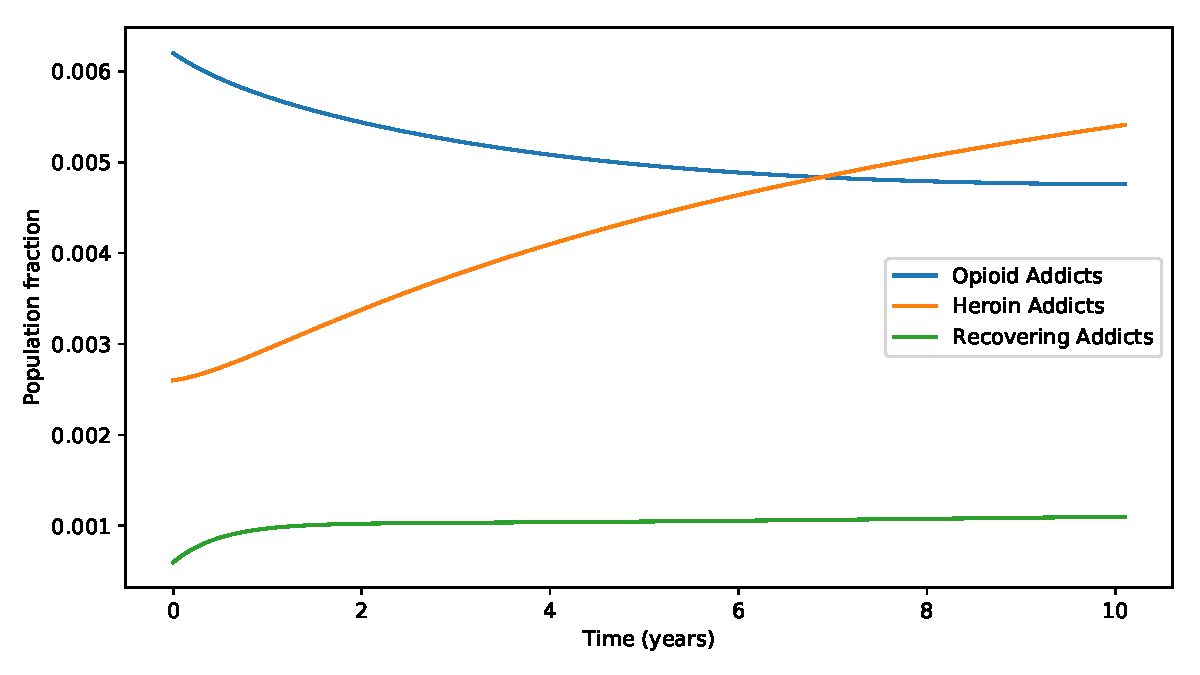
\includegraphics[height=6cm, width=11cm]{3_class_plot.pdf}

\end{frame}




\begin{frame}
\frametitle{Example Solution Curves}

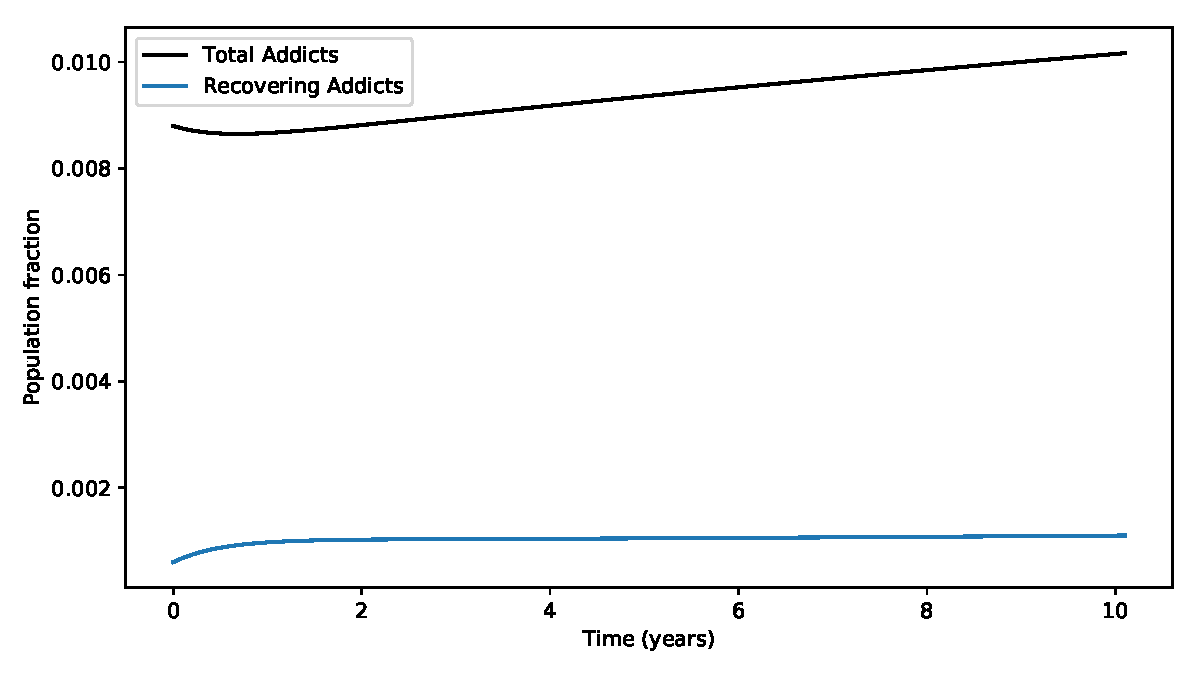
\includegraphics[height=6cm, width=11cm]{total_addicts_plot.pdf}

\end{frame}




\begin{frame}
\frametitle{Future Tasks/Possible Extensions}
\begin{itemize}
\item<1> Obtain local data from Knox County/East Tennessee and fit parameters to data. 
\vspace{.2cm}
\item<1> Perform sensitivity analysis to determine the sensitivity of each of the classes to the parameters (i.e. the contribution of each of the parameters to the sizes of the classes). 
\vspace{.2cm}
\item<1> Explore management strategies for how to best treat pain with prescriptions while reducing opioid addiction and heroin use.  
\end{itemize}
\end{frame}

\begin{frame}
\vspace{1cm}
\begin{center}
\large{Acknowledgements:}  \\
\vspace{0.5cm}
\large{Discussions with Dr. Nicholas Battista and Leigh Pearcy}
\end{center}
\end{frame}



\begin{frame}
\frametitle{Calculating $\mathscr{R}_0$ }
\begin{itemize}
\item<1>  Assuming A, H and R are the addicted compartments, and with $\gamma=0$ and $\xi=0$, we have the following matrices that meet the assumptions of the Next Generation Matrix Method: \\
\vspace{.5cm}
%\scriptsize
\begin{center}
$\mathscr{F}=$
$ \begin{pmatrix}

%0 \\
%0 \\
\beta SA \\
\theta_{1}SH+\theta_{2}PH \\
0
\end{pmatrix}$ \\ 
\end{center}
\vspace{.5cm}
\begin{center}
$\mathscr{V}=$
$ \begin{pmatrix}

%\alpha S + \beta SA+\theta_{1}SH-\epsilon P-\delta R-\mu(P+R+A+H)-\mu_{A}A-\mu_{H}H \\
%-\alpha S+\epsilon P +\theta_{2} PH +\mu P \\
-\sigma_{A}R+\zeta A+\theta_{3} AH + (\mu +\mu_{A})A \\
-\theta_{3}AH-\sigma_{H}R+\nu H +(\mu +\mu_{H}) H \\
-\zeta A -\nu H +\delta R +\sigma_{A}R +\sigma_{H}R +\mu R\\
\end{pmatrix}$.
\end{center}
\end{itemize}
\end{frame}



\begin{frame}
\frametitle{Calculating $\mathscr{R}_0$ }
\begin{itemize}
\item<1> Taking $F=\frac{\partial \mathscr{F}_i}{\partial x_j} (0, y_0)$ and $V=\frac{\partial \mathscr{V}_i}{\partial x_j} (0, y_0)$, i, j$=1,2,3$, where \\ (0, $y_{0}$) $=(\frac{\epsilon + \mu}{\alpha + \epsilon +\mu},\frac{\alpha}{\alpha + \epsilon +\mu},0,0,0)$ is the addiction-free equilibrium: \\

\begin{center}
$F=$
$ \begin{pmatrix}

\beta S^* &  0  & 0 \\
0 & \theta_1 S^* +\theta_2 P^* & 0\\
0  &   0 & 0\\
\end{pmatrix}$


\vspace{.3cm}
$V=$
$ \begin{pmatrix}

\zeta +\mu +\mu_A &  0  & -\sigma_A \\
0 &  \nu+\mu+\mu_H & -\sigma_H\\
-\zeta& -\nu  & \delta + \sigma_A + \sigma_H + \mu\\

\end{pmatrix}$.
\end{center}
\end{itemize}
\end{frame}





\begin{frame}
\frametitle{References of other models}
\begin{enumerate}[-]
\scriptsize 
\item Driessche, P. v. d. and Watmough, J. (2008). Mathematical Epidemiology, chapter 6: Further Notes on the Basic Reproduction Number, pages 159?178. Springer, Berlin, Heidelberg.
\item (2017). HHS acting secretary declares public health emergency to address national opioid crisis.
\item National Institute on Drug Abuse (NIDA) Prescription Opioids and Heroin. d14rmgtrwzf5a.cloudfront.net/sites/default/files/19774-prescription-opioids-and-heroin.pdf
\end{enumerate}

Previous heroin models: 
\begin{enumerate}[-]
\scriptsize
\item White, E. and Comiskey, C. (2007). Heroin epidemics, treatment and ode modelling. Mathematical Biosciences, 208:312?324.
\item Liu, J. and Zhang, T. (2011). Global behaviour of a heroin epidemic model with distributed delays. Applied Mathematics Letters, 24:1685?1692.
\end{enumerate}
\end{frame}




\end{document}